\documentclass[a4paper, 12pt]{article}

% This file contains global setup commands so that we can write in our main document without cluttering up the workspace. This file is the first thing included in the main paper after the \documentclass command, and all settings are immediately available.

\usepackage{graphicx}
\usepackage{xcolor}
\usepackage{parskip}
\usepackage{wrapfig}
\usepackage{amsmath}

% Font settings
\usepackage{fontspec}
\usepackage{titlesec}
\usepackage{titling}
\setmainfont{Open Sans}
\newfontfamily \headingfont[]{Open Sans Light}
\newfontfamily \codefont[NFSSFamily=JetBrainsMono]{JetBrains Mono}
\definecolor{accent}{rgb}{0.8, 0.0, 0.0}
\titleformat{\section}
	{\Huge\headingfont}{\thesection}{1em}{}[{\color{accent}\titlerule[4pt]}]
\titleformat{\subsection}
	{\Large\headingfont}{\thesection}{1em}{}[{\color{accent}\titlerule[2pt]}]
\titleformat{\subsubsection}
	{\large\headingfont}{\thesection}{1em}{}[{\color{accent}\titlerule[1pt]}]
\setmonofont{JetBrains Mono}
% Set to clear page before each section.
\newcommand{\sectionbreak}{\clearpage}

% Link settings
\usepackage{hyperref}
\definecolor{linkcolour}{rgb}{0.7, 0.133, 0.133}
\hypersetup{
	colorlinks,
	breaklinks,
	urlcolor=linkcolour,
	linkcolor=linkcolour,
	citecolor=linkcolour
}

% Code settings
\usepackage{minted}
\usepackage[htt]{hyphenat}

% Note: For some reason, this patch is needed to allow minted to work with python3, since it just looks for "python" by default.
\usepackage{xpatch}
\makeatletter
\xpatchcmd\minted@pygmentize
	{python -c}
	{python3 -c}
	{}{\fail}
\xpatchcmd\minted@autogobble
	{python -c}
	{python3 -c}
	{}{\fail}
\makeatother

\usemintedstyle{default}
\definecolor{codebg}{rgb}{0.973, 0.973, 0.973}
\definecolor{codehighlight}{rgb}{0.360, 0.215, 0.309}
\setminted{
	autogobble=true,
	encoding=utf-8,
	numbers=left,
	bgcolor=codebg,
	highlightcolor=codehighlight,
	fontfamily=JetBrainsMono,
	fontsize=\scriptsize,
	breaklines,
	tabsize=2
}
\renewcommand{\theFancyVerbLine}{\sffamily{\scriptsize\oldstylenums{\arabic{FancyVerbLine}}}}

% Header/Footer settings
\usepackage{fancyhdr}
\usepackage{lastpage}
\usepackage[left=3cm, right=3cm, top=2cm, bottom=4cm]{geometry}
\pagestyle{fancy}
\fancyhead[L,C,R]{}
\renewcommand{\headrulewidth}{0pt}
% Footer definition
\fancyfoot[L]{
	
\includegraphics[width=2cm]{img/rug_icon.jpg}
}
\fancyfoot[C]{}
\fancyfoot[R]{
	\headingfont
	\large
	Page \thepage\ of \pageref*{LastPage}
	\normalfont
	\normalsize
}

% Bibiliography settings
\usepackage[
	backend=bibtex,
	style=numeric,
	natbib=true,
	autocite=superscript
]{biblatex}
\addbibresource{sources.bib}

\setcounter{secnumdepth}{-3}
\setcounter{tocdepth}{2}

\begin{document}

% This file defines the title page formatting.

\begin{titlepage}
	\headingfont
	\begin{center}
		\LARGE \textbf{On the Efficacy of Keyword Searches to Find Meaningful Architectural Knowledge in Open-Source Software Mailing Lists}
		
		\vspace{0.5cm}
		
		\Large
		Bachelor Thesis for Computing Science
		
		\vspace{2cm}
		
		\begin{tabular}{l r}
			\Large \textbf{Andrew Lalis} & \footnotesize\href{mailto:andrewlalisofficial@gmail.com}{andrewlalisofficial@gmail.com} \\
			\footnotesize Supervised by \normalsize\textbf{Dr. Mohamed Soliman} & \footnotesize\href{mailto:m.a.m.soliman@rug.nl}{m.a.m.soliman@rug.nl}
		\end{tabular}
		
		
		\vspace{1cm}
		
		\small
		\normalfont
		\today
		
		\vfill
				
		
\includegraphics[width=\textwidth]{img/rug_fse_logo.png}
	\end{center}

	% Reset settings after we're done.
	\normalfont
	\normalsize
\end{titlepage}

\section{Abstract}
	Google and other web-based search engines give users immediate access to a plethora of knowledge. Mailing lists however, go unnoticed, and in searching for knowledge about software architecture for making important design decisions, they present an ideal source of information. In this study, we prepare the tools necessary to fetch, process, and categorize the architectural design decisions found in the mailing lists of several open-source projects from the Apache Software Foundation. An analysis will present information on the types of decisions, their prevalence, and the patterns these decisions form through a thread of emails. Several keyword-based search queries will be evaluated against the dataset to determine their effectiveness at retrieving the most relevant information.

{% Use a separate format for the table of contents.
	\hypersetup{linkcolor=black}
	\headingfont
	\tableofcontents
}

\section{Introduction}
	In this paper, we'll explore the efficacy of using targeted keyword search queries to find architectural knowledge in mailing lists for open-source software projects. More simply put, we'll build tools, collect data, and analyze that data to qualitatively determine how effective certain keyword-based search queries are at finding useful information in large sets of emails, sent in mailing lists for developers to communicate about large open-source software projects.
	
	\subsection{Software Architecture}
		Behind every software system you interact with, including the one used to read this paper, is a set of elements, relationships, and rationale that define the software's architecture. While on the surface, you see the \textit{implementation} of the software, the \textit{architecture} is concerned with what elements, their interactions in order to provide a framework for satisfying the requirements of the system \cite{perry}. Continuing our example, the software you're using to read this paper probably uses an architecture that includes elements like a PDF renderer, file reader, and a controller to manage your button clicks and mouse scrolling. Collectively, this set of components, design decisions, rationale, assumptions, and context together are defined as the \textit{architectural knowledge} of the system\cite{denboon}.
		
		In Perry's 1992 paper, "Foundations for the Study of Software Architecture", he posits that "we have not yet arrived at the stage where we have a standard set of architectural styles with their accompanying design elements and formal arrangements," and that each system is "a new architecture" \cite{perry}. While we are perhaps nearer now, 30 years later, to that mythical stage of architectural standardization, indeed many new systems are genuinely new architectures, with new elements or entirely novel approaches to communicating between components, where engineers must consult both their acquired skills and the collective knowledge of their peers, to make a best-effort to build a system to satisfy their requirements.
		
		Despite the plethora of resources available to the modern software engineer, we still often see \textit{architectural knowledge vaporization}\cite{jansen} because of undocumented decisions engineers took when designing the architecture of a system, or because it's impossible or practically infeasible to extract useful information. This dissipation of knowledge is a function of time and architecture size, and can lead to some serious problems that have already established themselves as hallmarks of poor software design in the industry, such as an increasing cost to improve or upgrade a system \cite{jansen, perry}, and a lack of reusability \cite{jansen}, and an increased cost of maintenance \cite{randell} even when no new features are added. These costs can, and often do, reach a point at which it is simply more effective to start over, abandoning completely any established work on an architecture. Through the years, this evolved from reprogramming low-level batch programs for early computing installations\cite{randell}, to today's distributed systems. Succinctly, a loss of architectural knowledge, by conjecture, leads to a loss of value and a loss of efficiency, and this paper aims to add additional tools to our collective defense against such regression.
		
	\subsection{Searching}
		It is important to explore different avenues for acquiring knowledge, especially as the body of information grows exponentially with time. It is difficult for developers and software architects to make informed decisions about their own projects, because the source of their knowledge is distributed in a variety of disparate sources. If we can reliably glean information about software architecture and the successful (and unsuccessful) decisions that other field experts have made, we can make this knowledge more accessible for all.
		
		Most people are familiar with "googling" to find solutions to their questions, but Soliman et al. has shown that using web search engines is not effective for mining knowledge from mailing lists\cite{soliman}. This probably is a symptom of the fact that most search engines do not index emails sent in mailing lists (as it generally doesn't make sense to do so), and that search engines can't provide a friendly user experience for navigating results that would be shown from mailing lists.
		
		Therefore, we'll need to index and search over emails independently. Of course, this detaches the research from what the majority of people are doing in their everyday lives, but presents more opportunities for automated architectural knowledge scraping, and as Bhat et al. has shown, an effective machine learning model is well within the realm of possibility\cite{bhat}.
		
	\subsection{Defining Types of Design Decisions}
		\label{sec:design-decisions}
		Before we can begin searching for architectural knowledge in earnest, we must first exhaustively define the types of distinct architectural design decisions that will be categorized.
		
		We start by evaluating Kruchten's original set of design decisions in section 2.1 of "Building Up and Reasoning About Architectural Knowledge"\cite{kruchten}, which lists four main kinds of decisions: \textbf{existence}, \textbf{ban}, \textbf{property}, and \textbf{executive}.
		
		These decisions were conceived in a domain that must consider architectural knowledge from a large variety of sources, and so we also consult den Boon\cite{denboon} and Faroghi\cite{faroghi} for more information that's specific to open-source issue/ticket boards and mailing lists. From their more specific lists, as well as some cursory categorization attempts, the following architectural design decisions were adopted.
		
		\subsubsection{\textbf{Existence}}
			Existence decisions are those that are concerned with the creation of new elements of a system's conceptual or implementation architecture, or the creation of behavioral connections between existing components. Generally, existence decisions manifest themselves in discussions about whether to add a new component to a system, or to link components together.
			
			\textit{Structural} decisions are a subset of existence decisions that focus solely on the creation or modification of components of an architecture; most often the addition of new components to a system.
			
			On the other hand, \textit{behavioral} existence decisions are concerned with, well, the behavior of the components of a system, namely how multiple components in a system interact with each other.
			
			For example,
			\begin{itemize}
				\item The system shall incorporate an additional process manager to orchestrate other high-level tasks.
				\item The system shall send periodic "heartbeat" packets to connected subsystems.
			\end{itemize}
		
		\subsubsection{\textbf{Property}}
			This category of design decision is taken almost verbatim from Kruchten's originally proposed list of architectural design decisions\cite{kruchten}, and is defined as one which states an enduring, overarching trait or quality of the system. This is not so much related to any particular element or behavior because they often necessarily affect many components with cross-cutting concerns.
			
			For example,
			\begin{itemize}
				\item The system shall be able to process at least 10,000 incoming connections concurrently.
				\item The system shall allow for flexible third-party plugin integration.
			\end{itemize}
		
		\subsubsection{\textbf{Process}}
			Again, this design decision is taken without much need for revision, from previous papers on the subject. A process decision is concerned less with the architecture itself, and more the internal development process. This includes things like software quality and testing strategies, code review procedures, and enhancement proposal protocols.
			
			For example,
			\begin{itemize}
				\item We as developers should define a strict suite of tests that must pass in order for any new release to be made available to the public.
				\item We should create a formal procedure for submitting patch requests.
			\end{itemize}
		
		\subsubsection{\textbf{Technology}}
			These decisions are made regarding the comparison, evaluation, and choice of third-party technologies for use in or with an architecture. This could be as simple as discussing a choice of programming language, to choosing a set of supported Open-ID Connect API providers for a user authentication micro-service. Generally, an email shall be considered to contain a technology design "decision", even if no discrete decision is made in that email. This is because a large part of technology discussions focuses on evaluating the properties of various alternative solutions, and such discussions have been found in practice to end with a rather simple, abrupt choice based on a vote.
			
			For example,
			\begin{itemize}
				\item We would like to use the \textit{D} programming language to write startup scripts for the system, because of its flexible syntax and high performance\cite{bright}.
				\item Our development team should make a choice between using Jira or GitHub Issues for our ticket board. Here are their pros and cons: ...
			\end{itemize}
		
	\newpage
	\subsection{Research Questions}
		\label{sec:research-questions}
		The main research question that this paper attempts to answer is summarized in the following question:
		
		\large \textbf{What architectural knowledge exists in open-source software development mailing lists?}
		\normalsize
		
		This broad main question can be further segmented into a series of more specific questions on the nature of the knowledge that exists in mailing lists:
		
		\begin{enumerate}
			\item What types of architectural design decisions are present in mailing lists?
			\item How often do architectural design decisions appear in mailing lists?
			\item What patterns exist in the order in which architectural design decisions appear? Furthermore, why do such patterns, if any, exist?
			\item How effective is using Apache Lucene to index and search for architectural design decisions in mailing lists?
			% \item How can we use data gathered in this research to improve our search queries?
		\end{enumerate}
	
\section{Related Work}
	In the field of architectural knowledge acquisition (granted, a rather niche field), the work of this research builds directly on the results obtained in den Boon's paper that explored the effectiveness of using the Apache Lucene search engine for finding this knowledge\cite{denboon}. This research found that Lucene can indeed be used for finding knowledge effectively, and also provided a basis for the \hyperref[sec:queries]{four queries} that this study uses for searching. It also concluded that, when using these queries to search through both issue/ticket boards and mailing lists, that mailing lists were more suitable to finding "macro architectural design decisions".
	
	The primary supervisor of this paper, Mohamed Soliman, also prepared a study in 2021 that evaluated the effectiveness of common web search engines (i.e. \href{https://google.com}{Google}) to find architectural knowledge, and from this paper we can learn that there are some key drawbacks to such a "lazy" approach to searching for architectural knowledge using the world's most ubiquitous search engine: design decisions are underrepresented, issue trackers and mailing lists are not indexed by search engines, and that most actual open-source software architecture on websites like \href{https://github.com}{GitHub} is not easily accessed. Furthermore, we see from this paper that while Google \textit{does} make it easy to compare alternative solutions for architectural problems, with blogs and tutorials being the most common result, finding information on instantiating \textit{new architectures} is not as easily accessible. These drawbacks provide motivation to search for alternative, more targeted searches that go beyond Google's general purpose indexing patterns\cite{soliman}.
	
	Xiong et al. worked in 2018 on analyzing the content of open-source \href{https://hibernate.org/}{Hibernate} mailing lists to search for "assumptions regarding requirements, environment, design decisions, etc." and found that the Hibernate developer mailing list contained 832 such relevant results from a sample size of 9006 posts. This provides an indication that developer mailing lists can be a valid source of knowledge about architectural design decisions\cite{xiong}. As stated in that paper, this study attempts to address the need to "explore the feasibility of this study in other OSS projects". Similar to this, work done by Ding et al. shows definitively that discussions in OSS developer mailing lists \textit{do} lead to measurable changes in the software's architecture, which provides further indication that mailing lists have a high potential for finding legitimate, practical, and usable architectural knowledge\cite{ding}.
	
	Kruchten's paper "Building UP and Reasoning About Architectural Knowledge" provided a basis for the \textit{types} of architectural knowledge that this paper will discuss, particularly his discussion on the "Ontology of Design Decisions"\cite{kruchten}. This information is combined with the research of den Boon\cite{denboon} and Faroghi\cite{faroghi} to arrive at the formalized set of design decisions that is discussed in the \hyperref[sec:design-decisions]{Design Decisions} section of the methodology discussion.
	
	With regards to the development of the practical tools used for this study, Tang's comparative study of existing architectural management tools\cite{tang} was a useful indicator of what the current (well, as of 2008) functionalities and expectations are for such tools. However, the different solutions examined under that paper focused mainly on larger-scale commercial ventures, which this study is not. Those tools therefore had a plethora of additional requirements, like privileged access to architectural knowledge and concurrent user content locking. These features, while they can be useful when deployed in a large-scale setting, are not necessary for a simpler passive study of existing knowledge in mailing lists.
	
	To extend the discussion on tools for extracting knowledge, Bhat et al. managed to produce a machine learning model for the identification and classification of architectural design decisions in OSS issues, and managed to achieve 91.29\% accuracy in detection, and 82.79\% accuracy in classification\cite{bhat}. Granted, this model applies only to issues and not mailing lists, and mailing lists are generally more verbose, so the applicability of this study's findings to mailing list searching are rather limited. In any case, our study may help to provide data and guidance to future work on developing a machine learning model for the classification of emails, similar to Bhat's study.

\section{Tools}
	To facilitate the research described in this document, a suite of tools was developed to aid in the fetching, processing, categorization, and analysis of emails from various open-source mailing lists. This section contains a detailed overview of each of these tools, and a high-level overview of the system architecture and how the entire suite can be used from start to finish.
	
	The entire collection of tools and their source code is available online at the \href{https://github.com/ArchitecturalKnowledgeAnalysis}{Architectural Knowledge Analysis} GitHub organization. Each of the tools discussed in this section is organized under a separate repository. In general, any projects written in \textit{Java} require the user to have version 17 or greater installed to build the project or run any executables/apps produced by it. \href{https://adoptium.net/temurin/releases}{You can get the latest OpenJDK release here.} Any projects written in \textit{D} should use a fairly recent version of D. The DMD compiler, version 2.099.1, was used to build and run all D projects/scripts. \href{https://dlang.org/download.html}{You can get the latest D compiler here.}
	
	Note that, especially for D projects, development was done in a Linux environment, and no serious attempt was made to provide additional compatibility and support for the Windows or Mac operating systems. Any compatibility is simply a consequence of the cross-platform nature of the technologies used. File path separators, process management, permissions, and other functionalities are handled differently in other operating systems, thus it is encouraged that you use a Linux-based OS to make use of these tools.
	
	\subsection{Overview}
		While each of the tools described in this section exist as a standalone project that can be incorporated into any third-party application, the majority of these focus on providing auxiliary services to the \hyperref[sec:email-dataset-browser]{Email Dataset Browser} application.
		
		The general workflow that these tools enable, is described as follows:
		
		\begin{enumerate}
			\item Raw \texttt{mbox} files (files containing many emails) are downloaded from a mailing list archive's API.
			\item The mbox files are parsed to extract the individual emails and their metadata, and this is used to build a relational database and Lucene search index.
			\item A researcher categorizes the emails in the dataset according to a set of pre-defined criteria. In this case, we use the \hyperref[sec:design-decisions]{architectural design decisions} covered in the introduction.
			\item The categorized emails and Lucene search results are exported from the dataset to a JSON format.
			\item Analysis is performed on the data and visualizations are generated.
		\end{enumerate}
	
	\newpage
	\subsection{Email Downloader}
		\label{sec:email-downloader}
		The email downloader component helps us to solve the first step of the workflow: fetching \texttt{mbox} files from a mailing list archive. It does this by introducing the \texttt{MailingListFetcher} that provides a common interface for fetching mailing list archives that is designed to be compatible with most online mbox file repositories. It simply defines a single \texttt{download} method that downloads a mailing list (identified by its domain and list name) and saves the mbox files to a given directory. The caller provides a start and end timestamp to limit the download to only those archives pertaining to emails sent within the specified timeframe, and finally a message consumer that can be used for downloader to report messages as it performs the download.
		
		\begin{minted}[numbers=none]{java}
CompletableFuture<Collection<Path>> download(
	Path dir,
	String domain,
	String listName,
	ZonedDateTime start,
	ZonedDateTime end,
	Consumer<String> messageConsumer
);
		\end{minted}
	
		The download happens asynchronously, and the returned \texttt{CompletableFuture} is completed when the download is complete.
		
		Because this research will focus on mailing lists from the Apache Software Foundation, we provide an \texttt{ApacheMailingListFetcher} implementation that implements the above interface. It uses Apache's (undocumented) API endpoint at \href{https://lists.apache.org/api/mbox.lua}{https://lists.apache.org/api/mbox.lua} to download emails via HTTP, using a rate-limited strategy with a delay of 1 second, and a short-circuiting behavior where the fetcher will give up after 10 consecutive months of no emails.
		
		For example, we could request the following from the API:
		
		\begin{minted}[numbers=none]{bash}
curl https://lists.apache.org/api/mbox.lua?domain=nemo.apache.org&list=dev&d=2007-12
		\end{minted}
		
		Here, we fetch all emails (in a single mbox file format) from the \textit{dev} list in the Apache Nemo project from the month of December, in 2007. The API will respond with a file download, which our library saves to the system's drive (in the desired directory).
		
		\subsubsection{CLI}
			Besides the programmatic interface that the email downloader provides, it also provides a command-line interface when running the project's JAR file as an executable. The JAR file can be obtained from the project's \href{https://github.com/ArchitecturalKnowledgeAnalysis/EmailDownloader/releases}{releases} page, or built from source using maven:
			
			\begin{minted}[numbers=none]{bash}
mvn clean package assembly:single
			\end{minted}
		
			The CLI provides access to, at the time of writing, just the Apache implementation for the mailing list fetcher, and essentially allows one to invoke the \texttt{download} method from the command-line. Its detailed usage information is provided below.
			
			\begin{minted}[numbers=none]{text}
Usage: EmailDownloader [-hV] -d=<domainName> [--from=<fromDate>] -l=<listName>
                       [-o=<outputDir>] [--until=<untilDate>]
  -d=<domainName>            The domain to download from. For example, "hadoop.
                               apache.org"
  --from=<fromDate>          Earliest period to download from, inclusive.
                               Formatted as yyyy-mm.
  -h, --help                 Show this help message and exit.
  -l=<listName>              Name of the mailing list to download from.
  -o, --output=<outputDir>   Directory to place downloaded files in. Will
                               create it if it doesn't exist.
  --until=<untilDate>        Latest period to download from, inclusive.
                               Formatted as yyyy-mm.
-V, --version                Print version information and exit.
			\end{minted}
		
			This information is also available via the standard \texttt{--help} flag.
	
	\newpage
	\subsection{MBox Parser}
		\label{sec:mbox-parser}
		With the raw mbox files obtained by the email downloader, it's not yet possible to do anything productive until we extract the individual emails and their data. To do this, we introduce the MBox Parser library. This library provides a programmatic method for extracting and pre-processing emails from all mbox files in one or more directories or files.
		
		The main interface is the \texttt{MBoxParser} class, from which objects can be instantiated with a provided \texttt{EmailHandler} implementation that executes a callback for each email parsed from the set of mbox files. Specifically, the format for emails obtained by the parser is as follows:
		
		\begin{minted}[numbers=none]{java}
public class Email {
	public String messageId;
	public String inReplyTo;
	public String sentFrom;
	public String subject;
	public ZonedDateTime date;
	public String mimeType;
	public String charset;
	public String transferEncoding;
	public byte[] body;
}
		\end{minted}
	
		Additionally, a utility method is provided to read the body of the email as a simple string. Internally, the parser makes use of Apache's \href{https://james.apache.org/mime4j/}{Mime4j} library, and a custom email content handler that performs some extra processing on email dates and message ids to improve uniformity:
		
		\begin{itemize}
			\item We expect dates in the RFC-1123 format. For example, \texttt{Sun, 21 Oct 2018 12:16:24 GMT}, and if we get something slightly different, attempts are made to transform it into an acceptable format.
			\item We strip the angle brackets (\texttt{<} and \texttt{>}) from the email's unique message id. These brackets exist on every email, and do not contribute to the uniqueness of the id. Stripping them makes the message ids more readable as plain text when embedded in HTML or any XML, and makes searching over them easier.
		\end{itemize}

		The Mbox Parser provides users with the ability to provide their own filter functions to further refine the results, but this will be discussed in more detail when explaining the Email Indexer component. No command-line interface is provided for this library; it is only available as a programmatic Java library, meant to be used in concert with the email downloader and any other programs that consume individual emails.
	
	\newpage
	\subsection{Email Indexer}
		\label{sec:email-indexer}
		While the downloader and parser can be thought of as auxiliary to the goals of this research, the Email Indexer project forms the core of the email dataset's structure, and by implication, the research in this paper. The email indexer is a Java library that offers a programmatic interface for creating, managing, and exporting categorized email data.
		
		Each dataset produced by the email indexer exists nominally as a directory, or as a ZIP archive of a directory. Each dataset directory contains the following components:
		
		\begin{enumerate}
			\item An embedded relational \href{https://www.h2database.com}{H2 database} file named \texttt{database.mv.db}, which stores all emails, tags, and other key information for the dataset. A \hyperref[fig:schema]{schema diagram} is provided in this section, and the full schema definition can be found \hyperref[sec:dataset-schema]{in the appendix}.
			\item An \texttt{index} directory in which the indexes generated by \href{https://lucene.apache.org/}{Apache Lucene} are stored.
			\item A \texttt{metadata.properties} file that holds some meta information about the dataset. As of the time of writing, the only metadata stored in this file is the dataset version, which, again at the time of writing, is version 2.
		\end{enumerate}
	
		\subsubsection{Email Thread Structure}
			\begin{wrapfigure}{r}{0.4\textwidth}
				\label{fig:email-threads}
				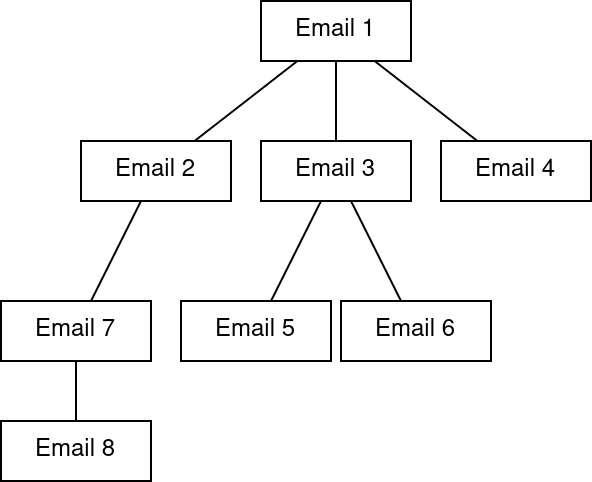
\includegraphics[width=0.4\textwidth]{img/email-threads.png}
			\end{wrapfigure}
			
			Emails have a self-referencing \textit{many-to-one} relationship defined by their "In-Reply-To" field. It is important to understand the consequences of this structure, and how it impacts the dynamics of processing data. In any information system, a self-referencing, many-to-one relationship that an entity participates in, can be interpreted as a \textit{tree} data structure.
			
			Each email can be thought of as a node in the tree, where each reply to that email forms a branch. There is no limit to how wide or deep the tree can become, because there is no universal hard limit on the number of replies to an email, nor on how many replies may be sent in a thread.
			
			In previous research by den Boon, this natural tree structure of email threads was artificially flattened into a sequential list, presumably to facilitate more efficient methods of working with the data\cite{denboon}. However, in this research, the tree structure of the emails is preserved in the dataset, because it more accurately depicts how real users would navigate a set of emails using any number of existing programs, and therefore can provide a better model for determining the effectiveness of searches. This choice does come with some drawbacks, however.
			
			\begin{enumerate}
				\item Because emails form a tree structure, navigating the dataset is more computationally intensive, and more complex for a user, than if one could simply traverse a flat list.
				\item Analysis is more complex, due to the fact that most algorithms will need to incorporate tree traversal, either iteratively or recursively.
				\item Relational databases generally do not offer facilities for recursive fetching, which can lead to performance losses when processing large sets of emails.
			\end{enumerate}
			
			Despite the drawbacks, it is important to analyze and categorize emails in a format that does not lose the latent structural information contained in the email thread's tree itself. Furthermore, for this particular research, the volume of data and methods of analysis do not present any difficulties in terms of computational performance.
		
		\subsubsection{Database Schema}
			\begin{wrapfigure}[16]{r}{0.5\textwidth}
				\label{fig:schema}
				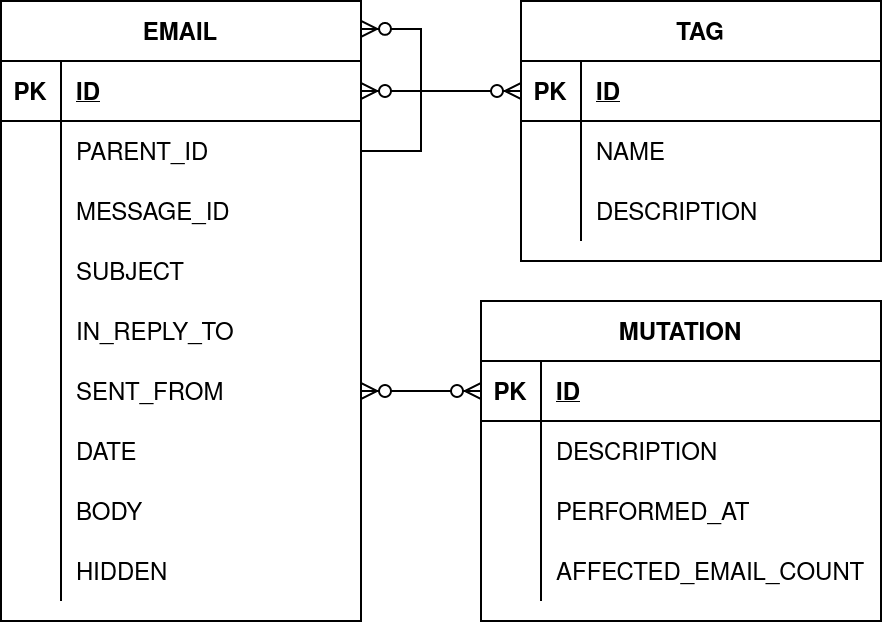
\includegraphics[width=0.5\textwidth]{img/simple_schema.png}
				\caption{A diagrammatic representation of the email dataset's relational schema.}
			\end{wrapfigure}
			The relational schema is the core of the email dataset, and defines how we operate on and organize the data. It is purposefully designed to be as simple as possible, to make it easy to use the dataset in a variety of applications and environments.
			
			The schema consists of three entities: \textit{emails}, \textit{tags}, and \textit{mutations} (although mutations are not strictly required).
			
			\textbf{Emails} are, as you'd probably expect, the entity that represents a single email message, sent by someone, in a mailing list. While emails \textit{do} have their own unique \texttt{MESSAGE\_ID} attribute\cite{rfc5322}, they are identified by an 8-byte integer primary key. This reduces the dataset size, improves search performance due to the monotonic nature of incrementing primary keys, and allows for easier referencing of emails by their id, instead of a long, randomly-generated message id.
			
			Also of note is an email's \texttt{PARENT\_ID}, which is a self-referencing foreign key that references another email entity by its id. This foreign key is the manifestation of the \textit{many-to-one} relationship between an email and its parent, where many "child" emails may refer to one parent email. The parent id is derived, when processing emails, from the email's "In-Reply-To" field. According to RFC 5322, the in-reply-to field, if present, must reference another email's message-id, and this format of replies forms the basis of an email thread's structure\cite{rfc5322}.
			
			\textbf{Tags} are entities which can be attached to any number of emails, to offer a method of categorizing emails. Originally in version 1 of the dataset format, tags were not entities but simple texts that were attached to each email, but it was discovered during the development of the tools for this research that there are several benefits to having tags as their own entities: the ability to edit a tag's name, provide a description, and reduce the total dataset size by referencing an 4-byte integer id instead of keeping a copy of a string for each tag applied to an email.
			
			There exists a \textit{many-to-many} relationship between \textbf{emails} and \textbf{tags}, which one could verbalize as, "A tag may be applied to many emails, and an email may have many tags applied to it."
			
			\textbf{Mutations} are entities that record some change to the dataset which is used as a historical record of how a the emails in a dataset are filtered or modified. Mutations are used at the discretion of any third-party application which interfaces with the EmailIndexer API, and are not required to be used.
			
			There exists a \textit{many-to-many} relationship between \textbf{mutations} and \textbf{emails}, which one could verbalize as, "A mutation may involve many emails, and an email may be involved in many mutations." It is not required that a mutation be linked to any emails.
		
		\subsubsection{Indexing with Lucene}
			Alongside the relational database resides the \texttt{index} directory, as mentioned at the start of this section. This contains the indexes produced by the \href{https://lucene.apache.org/}{Apache Lucene} indexing library when we build an index using the emails in the database. This index is then used for executing query searches over the database by users.
			
			For each email in the dataset, we index the following fields as non-stored string-type fields using the \texttt{DOCS\_AND\_FREQS\_AND\_POSITIONS} index options provided by Lucene\cite{apache-lucene}:
			\begin{itemize}
				\item The \texttt{SUBJECT} field.
				\item The \texttt{BODY} field.
			\end{itemize}
			In addition to these indexed fields, we store the email's id and pre-compute the \textit{root id} (id of the first email in the current email's thread), as these are essential for producing actionable results from any query search on the index.
	
		\newpage % To avoid breaking the title line.
		\subsubsection{Dataset Generation}
			Probably the most critical part of the email indexer is its workflow for taking in mbox files, using the Mbox Parser to extract emails, and build the dataset and its various components. The following snippet illustrates an abridged version of the dataset generation algorithm (with trivial log messages and typical Java verbosity removed).
			
			\begin{minted}{java}
public CompletableFuture<Void> generate(Collection<Path> mboxFileDirs, Path dsDir) {
	return Async.run(() -> {
		// Parse files and create database
		Files.createDirectories(dsDir);
		DatabaseGenerator dbGen = new DatabaseGenerator(dsDir.resolve("database"));
		List<Path> mboxFiles = new ArrayList<>();
		for (var dir : mboxFileDirs) {
			mboxFiles.addAll(findMboxFiles(dir));
		}
		MBoxParser parser = new MBoxParser(new SanitizingEmailHandler(dbGen));
		for (var file : mboxFiles) {
			parser.parse(file);
		}
		dbGen.postProcess(status);
		dbGen.close();
		
		// Generate Lucene Index
		EmailDataset dataset = new EmailDataset(dsDir);
		new EmailIndexGenerator().generateIndex(dataset);
		dataset.close().join();
		
		// Generate Metadata
		Properties props = new Properties();
		props.setProperty("version", "3");
		props.store(Files.newBufferedWriter(dataset.getMetadataFile()), null);
	});
}
			\end{minted}
			
			Notice on line 8 that we use a \texttt{SanitizingEmailHandler} to handle all parsed emails. This handler applies some extra sanitization to further reduce the amount of useless junk that ends up in the final dataset. It removes any emails which:
			\begin{itemize}
				\item Have an unknown charset (we're not able to decode them).
				\item Have a missing or empty body.
				\item Have a missing or empty message id.
			\end{itemize}
			Additionally, it also performs the following modifications to emails:
			\begin{itemize}
				\item Removes reply texts which start with "-----Original Message-----", or whose lines begin with ">". This greatly reduces the volume of text for large email threads, and helps to reduce the number of false-positives returned by searches.
				\item Strips "<" and ">" from the beginning and end of any email's message id, in-reply-to, or sent-from attributes.
			\end{itemize}
		
		\newpage % To avoid breaking the title line.
		\subsubsection{Data Access API}
			In order for the email indexer API to be used by third-party applications, we provided a set of \textit{repositories} that can be used to find, create, update, and delete entities from the dataset, as well as a set of \textit{searchers} that provide more advanced retrieval mechanisms with SQL and Lucene searching.
			
			\begin{enumerate}
				\item The \texttt{EmailRepository} provides access to emails, including methods to find both the full email entity, and a \textit{preview} which omits the body and in-reply-to fields to make it feasible for applications in search results or other scenarios where the full email information isn't needed.
				\item The \texttt{TagRepository} provides access to tags, and various methods for adding and removing tags from emails.
				\item The \texttt{EmailSearcher} has methods for finding emails using a collection of \texttt{SearchFilter}s, which are used to build SQL queries over the set of emails. The methods in the EmailSearcher generally return an \texttt{EmailSearchResult} which contains the actual email results, as well as some information that's useful for pagination implementations in third-party applications.
				\item The \texttt{EmailIndexSearcher} has methods for finding emails (or email threads) using an Apache Lucene search query.
			\end{enumerate}
		
			For developers' convenience, all data-access objects are full documented with accurate Javadoc so that the usage of the API is abundantly clear.
	
	\newpage
	\subsection{Email Dataset Browser}
		\label{sec:email-dataset-browser}
		The main part of the research, categorizing emails based on the types of architectural design decisions they contain, is accomplished by the Email Dataset Browser application. It is a desktop application built with Java and the Swing user-interface component library.
		
		While the original design is based on the \textit{ArchDetector} tool designed by den Boon\cite{denboon}, it was built anew to better support the structure of email threads, and provide a more extendable platform for analysis without needing to deploy a web server or PostgreSQL database like the ArchDetector did. Additionally, since den Boon's research, the Apache Software Foundation has updated their infrastructure for mailing list management, which broke the ArchDetector's automatic mailing list download functionality. Our Email Downloader tool addresses that.
		
		The browser is essentially a front-end for the Email Indexer's functionality, and provides some other conveniences. The remainder of this section will discuss all the features of the app, and how it is typically used for categorizing emails.
	
		\begin{figure}[H]
			\centering
			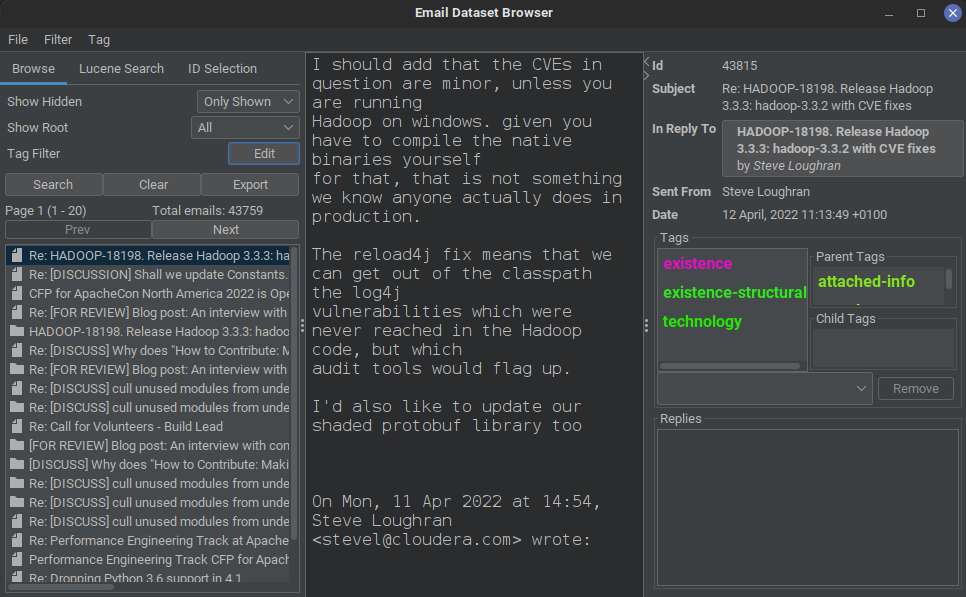
\includegraphics[width=\textwidth]{img/edb-app_populated.png}
			\caption{A screenshot of the email dataset browser app's main user interface, showing an email that has some tags.}
			\label{fig:edb-app-populated}
		\end{figure}
	
		\newpage
		\subsubsection{Generating a Dataset}
			\begin{wrapfigure}[14]{r}{0.5\textwidth}
				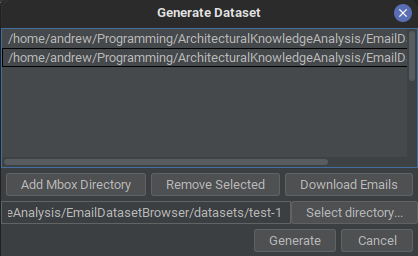
\includegraphics[width=0.5\textwidth]{img/edb-app_generate-dataset-popup.png}
				\caption{The popup for generating a new dataset.}
				\label{fig:edb-app-generate-dataset}
			\end{wrapfigure}
			The browser app allows users to generate a new email dataset from mbox files on the user's file system, and allows users to download mbox files on-the-fly from Apache's mailing lists. Navigate in the app's menu to \textbf{File} and then \textbf{Generate Dataset}, and you should see a popup open, as shown in figure \ref{fig:edb-app-generate-dataset}. The main interface consists of a list of directories to read mbox files from. You can add and remove directories from this list.
			
			\begin{wrapfigure}[18]{r}{0.4\textwidth}
				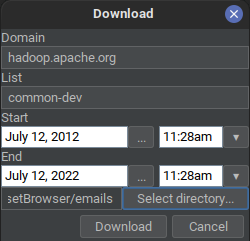
\includegraphics[width=0.4\textwidth]{img/edb-app_download-popup.png}
				\caption{The popup for downloading mbox files from Apache mailing lists.}
				\label{fig:edb-app-download-emails}
			\end{wrapfigure}
		
			If you'd like to download mbox files from Apache's mailing lists, you can use the \textbf{Download Emails} button to bring up another popup, as shown in figure \ref{fig:edb-app-download-emails}. In this interface, the user can provide the domain and list names, as discussed in the Email Indexer's section, as well as a start and end date and directory to download to. Do note that download can take a significant amount of time (up to 10 or 20 minutes for large mailing lists), so be patient with this step.
			
			Once you've downloaded and/or located all the directories containing mbox files you'd like to include in the dataset, you must select a directory in which to place the dataset. This directory will be populated with the dataset's database file, metadata file, and Lucene index directory. When you've done this, click \textbf{Generate} to generate the dataset.
			
			Again, this process may take a while, depending on the size of the dataset and your system's hardware performance, so please be patient. A popup will appear that shows messages from the email indexer's dataset generation system to indicate the current status as the process progresses. Once the generation is complete, you can click the \textbf{Done} button to exit the popup. The dataset now exists on your system, in the directory you specified in the popup, and you can open it like you would any other dataset using the app.
			
		\newpage
		\subsubsection{Opening and Browsing Datasets}
			To open a dataset, navigate to the \textbf{File} menu, and select \textbf{Open Dataset}. In this file selection dialog, select the a dataset's directory to open it. You may also select a ZIP archive file instead, in which case the app will first unzip the archive to a directory of the same name, and open that. Once you open a dataset, you'll see on your left a panel with three tabs labelled \textit{Browse}, \textit{Lucene Search}, and \textit{ID Selection}. These are the three different ways in which you can navigate the dataset.
			
			\begin{figure}[h]
				\centering
				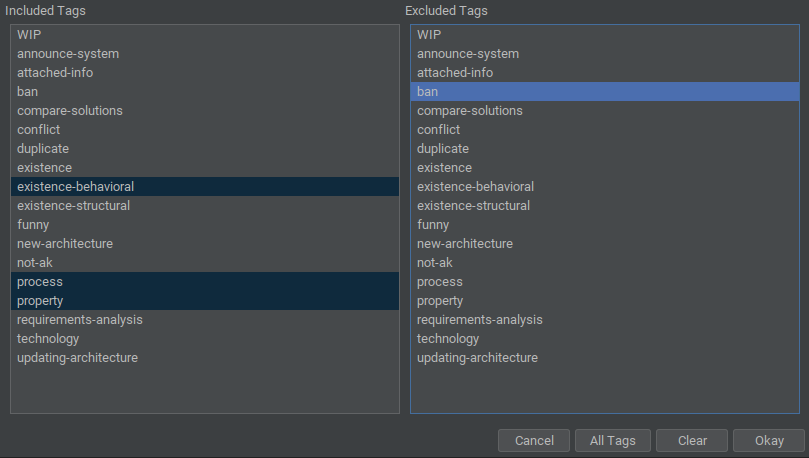
\includegraphics[width=0.8\textwidth]{img/edb-app_tag-filter-popup.png}
				\caption{Use this popup to filter emails in the standard browse panel based on the tags that they do or do not have.}
				\label{fig:edb-app-tag-filter}
			\end{figure}
		
			\begin{wrapfigure}[19]{l}{0.4\textwidth}
				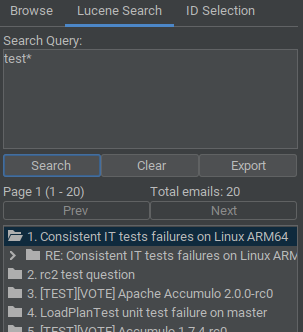
\includegraphics[width=0.4\textwidth]{img/edb-app_lucene-search-narrow.png}
				\caption{The view for searching the dataset using Lucene queries.}
				\label{fig:edb-app-lucene-search}
			\end{wrapfigure}
		
			In the \textit{Browse} view, you can browse the emails using a traditional paginated, filterable view. You can choose to show only hidden emails (those that have been removed by a user because they're irrelevant), only non-hidden emails (the default option), or both. You can also choose to show only \textit{root} emails, (emails that are at the root of an email thread, i.e. the first email in the thread), only child emails, or both (the default option). Finally, you can also filter the emails based on the tags they have, using the tag filter shown in figure \ref{fig:edb-app-tag-filter}. If you select tags under the \textit{Included Tags} list, only emails that have those tags will be shown. Conversely, if you select tags under the \textit{Excluded Tags} list, only emails which \textbf{do not} have those tags will be shown.
			

		
			In the \textit{Lucene Search} view, you can search the dataset using a provided Lucene query. You can read about the acceptable syntax for such queries in the \href{https://lucene.apache.org/core/9_1_0/queryparser/org/apache/lucene/queryparser/classic/package-summary.html}{Lucene 9.1 documentation}. Figure \ref{fig:edb-app-lucene-search} shows an example where we search over a dataset using the query "test*". The results show the list of all email threads which match the query, ranked from most to least relevant, according to Lucene. By default, only 20 results are shown, but this can be changed in the \textbf{Settings} under the \textbf{File} menu; look for the \texttt{Browse page size} option.
			
			\begin{wrapfigure}[18]{l}{0.4\textwidth}
				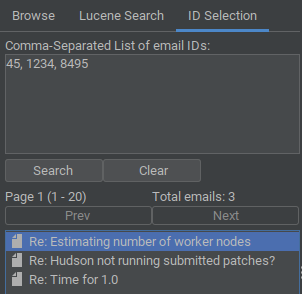
\includegraphics[width=0.4\textwidth]{img/edb-app_id-selection.png}
				\caption{The view for searching the dataset using specific email ids.}
				\label{fig:edb-app-id-selection}
			\end{wrapfigure}
		
			Finally, in the \textit{ID Selection} view, you may enter a comma-separated list of email ids, to view only those emails. Take note that by \textit{id}, we mean the id which the email indexer has assigned to the email when inserting it into the database, \textbf{not} the email's message id. As shown in figure \ref{fig:edb-app-populated}, the id can be found at the top of the email's information panel on the right-hand side of the app. This view is especially useful for the iterative process of familiarizing oneself with the types of architectural design decisions, and how they appear in various emails in practice.
			
			\begin{wrapfigure}[10]{r}{0.4\textwidth}
				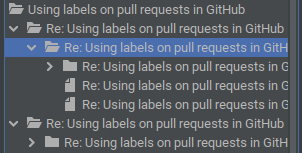
\includegraphics[width=0.4\textwidth]{img/edb-app_email-tree-view.png}
				\caption{The tree view used to navigate lists of emails.}
				\label{fig:edb-app-tree-view}
			\end{wrapfigure}
			
			In each of the three views, a list of emails is shown in the \textit{email tree view} below the view-specific options panel. As shown in figure \ref{fig:edb-app-tree-view}, this tree view allows the user to expand an email to show its replies, if any exist. With this type of view, it's easy to navigate large email threads, and get an overview of the high-level structure of the thread. Each email is listed in the view using its subject, similar to how many email client programs already do.
		
			Beside each email is shown an \textit{info panel} with detailed information about the selected email, as shown in figure \ref{fig:edb-app-info-panel}. This panel is shown beside each selected email, and can be expanded or hidden using the controls on the vertical divider between it and the email's main content view. Here you can see the following information, listed in the order in which it appears:
			
			\begin{enumerate}
				\item The email's assigned id. This is used in the ID Selection view.
				\item The email's full subject field.
				\item A link to the email that this one is a reply to, if any.
				\item The name of the person who sent the email.
				\item The date at which the email was sent.
				\item A panel which shows all the tags that have been assigned to the email. This will be covered more later.
				\item A list of replies to the email. You can click on a reply to navigate to it.
			\end{enumerate}
		
			\begin{wrapfigure}[20]{r}{0.5\textwidth}
				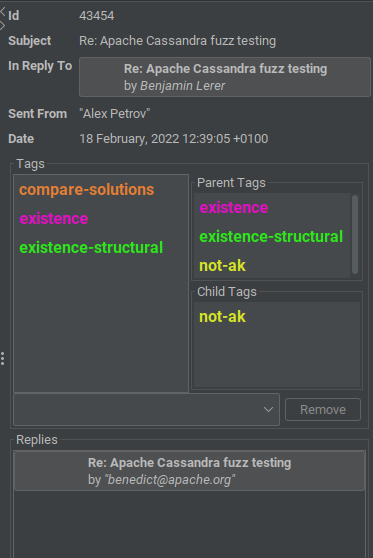
\includegraphics[width=0.5\textwidth]{img/edb-app_info-panel.png}
				\caption{The information panel that's shown beside each email.}
				\label{fig:edb-app-info-panel}
			\end{wrapfigure}
		
			In the email's \textit{tag panel}, you can see all the tags that have been assigned to the email. On the right, you can see the \textit{parent tags} (any tags that belong to any parent email of this one) and the \textit{child tags} (any tags that belong to any child email of this one). Each tag is colored using a random color derived from a hash of the tag's name, to improve readability and easy identification of tags.
			
			At the bottom of the tag panel, there's a select box where you can select tags to apply to the selected email. If you select any of the tags in the email's main list of tags, you can also click the \textbf{Remove} button to remove those tags. You can double-click on any of the tag items in any of the lists (main, parent, child) to edit the tag's name or description.
	
		\newpage
		\subsubsection{Managing Tags}
			\begin{figure}[h]
				\centering
				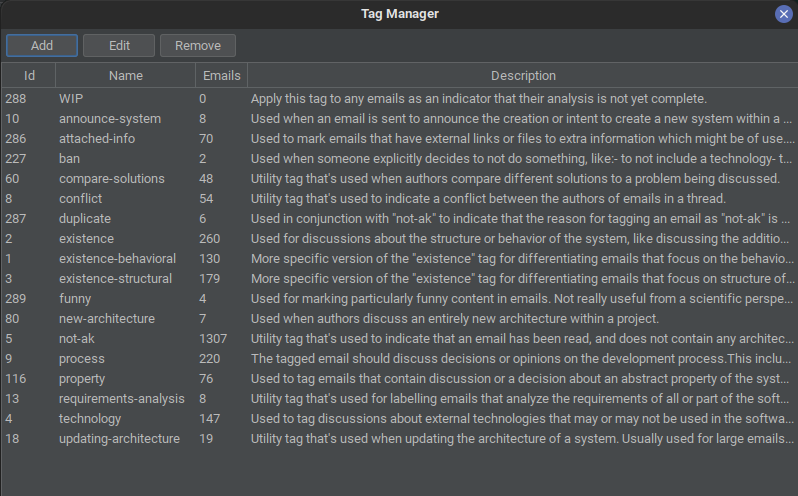
\includegraphics[width=0.8\textwidth]{img/edb-app_tag-manager.png}
				\caption{The tag manager popup, which shows a list of all tags and some information about them.}
				\label{fig:edb-app-tag-manager}
			\end{figure}
			
			To create, edit, or remove the set of tags that are available for applying to emails, you can use the \textit{tag manager}. Open this popup by navigating to the \textbf{Tag} menu, and select \textbf{Manage Tags}. You should see the popup shown in figure \ref{fig:edb-app-tag-manager}. Here, you can see a table showing all tags currently in the dataset. You can select a tag and click \textbf{Edit}, or just double-click it to edit. New tags can be added via the \textbf{Add} button, and selected tags can be removed via the \textbf{Remove} button. 
			
			\footnotesize
			Do take care with removal though, as removing a tag is a permanent and irreversible operation that will permanently remove information from your dataset. Consider renaming a tag to have an "unused" prefix first, until you're absolutely certain that a tag can be removed without losing any valuable information.
			\normalsize
			
		\subsubsection{Filtering Emails}
			While our APIs make a best attempt to remove some of the most egregious ill-formatted and useless emails, a large amount of noise does make it through to the dataset. Therefore, we provide a suite of tools to filter out emails using a few different methods. These are available in the \textbf{Filter} menu of the app.
			
			First, any email can be individually hidden with the \textbf{Hide} and \textbf{Show} buttons. Besides that, you can also hide all emails sent by the same author as the one who sent the selected email, or hide all emails that have exactly the same body content as the selected email, with \textbf{Hide by Author} and \textbf{Hide all by body} respectively. Finally, \textbf{Hide by SQL} can be used to manually define an SQL clause to hide all emails that match that clause.
	
	\newpage
	\subsection{Email Dataset Report Generator}
		\label{sec:email-dataset-report-generator}
		When enough data has been collected through the categorization of emails in a dataset, the dataset report generator pipeline is used to extract, analyze, and visualize the data. This pipeline is orchestrated by a \texttt{run\_pipeline.d} script that invokes each of the sub-processes in the correct order.
		
		This pipeline uses Java 17 with Maven, and D 2.099.1 with the Dub package manager. Additionally, it makes use of the \href{https://github.com/andrewlalis/dsh}{DSH} library for D. It's not required to have it installed, but it does make it easier to make changes to the pipeline script. You will need both Java and D, and their respective package managers installed to run the pipeline successfully. Additionally, the pipeline has not been validated on Windows or Mac operating systems. Use these at your own risk.
		
		\texttt{run\_pipeline.d}, or the \textit{pipeline runner} as it'll be referred to from now on, is an executable file that, if given the proper executable permissions, will run as-is. Otherwise, you can build the file using Dub as a single-file project. If using DSH, you can run the following command to compile a binary executable:
		
		\begin{minted}[numbers=none]{bash}
dshutil compile run_pipeline.d
		\end{minted}
	
		The pipeline runner, when run, expects a single argument, which determines the behavior of the program.
		
		\begin{itemize}
			\item If the \textbf{help} argument is passed, then a simple help message is shown.
			\item If the \textbf{clean} argument is passed, then files generated by previous runs are removed.
			\item If the \textbf{rebuild} argument is passed, then executable files for the various steps of the pipeline are rebuilt from source. Use this if you make changes to the source. Note that executables are also built automatically if they're missing at runtime.
			\item Otherwise, the argument is interpreted as the path to a \textbf{dataset directory} to run the pipeline on.
		\end{itemize}
		
		To summarize, the report generation pipeline is as follows:
		\begin{enumerate}
			\item Extract data from the dataset.
			\item Perform analysis on the data.
			\item Generate visualizations of the data.
		\end{enumerate}
		
		The remainder of this section will discuss each step of the pipeline in more detail.
		
		\newpage
		\subsubsection{Extraction}
			To extract the necessary data, a small Java program uses the Email Indexer as a dependency, and exports all emails that have any tag, into a large JSON array. Each email in the export is structured like so:
			\begin{minted}[numbers=none]{json}
{
	"id": 43815,
	"parent_id": 43810,
	"message_id": "CAL7CpJx7sSVZR+idVmdvwgDGX5DOD31L\u003d+fw@mail.gmail.com",
	"subject": "Re: HADOOP-18198. Release Hadoop 3.3.3: hadoop-3.3.2 with CVE fixes",
	"in_reply_to": "CAL7CpJydXGTxkgzV903dc2HR2yQgXpacs_iJa7MirKJQ@mail.gmail.com",
	"sent_from": "Steve Loughran \u003cstevel@cloudera.com.INVALID\u003e",
	"date": "2022-04-12T11:13:49+01:00",
	"body": "I should add that the CVEs...",
	"tags": [
		"existence",
		"existence-structural",
		"technology"
	]
}
			\end{minted}
			
			In addition to the emails, this program also exports information about various Lucene searches, because Lucene is inherently a Java library and this is our last opportunity to extract such data before the next steps of the pipeline. A list of queries is provided in the classpath of the program, in a \texttt{queries.properties} file. For each query, we get the list of individual emails and email threads that are returned as results, and compile this data into a JSON array.
			
			\begin{minted}[numbers=none]{json}
{
	"name": "decision_factors",
	"query": "actor* availab* budget* business case* client* concern* conform*",
	"threads": [39719, 42370, 42375],
	"emails": [43269, 42370, 42375]
}
			\end{minted}
		
			Finally, the program exports information about all known mutations to the dataset, and puts these into a JSON array. Below is an example of a mutation object.
			
			\begin{minted}[numbers=none]{json}
{
	"id": 6,
	"affected_email_count": 458,
	"description": "Hiding all emails sent by email addresses like: %hudson@lucene.zones.apache.or%"
}
			\end{minted}
		
			Thus the end result of this step is an \texttt{emails.json} containing the list of all tagged emails, a \texttt{searches.json} containing a list of all Lucene queries and the results they returned, and a \texttt{mutations.json} containing a list of all recorded mutations to the dataset.
			
			As an aside, we use the extraction step to opportunistically export and perform any additional steps besides core data extraction which can easily be done in Java. To that end, the extraction program also performs a minimalistic natural-language-processing pipeline on the set of tagged emails using Stanford's \href{https://stanfordnlp.github.io/CoreNLP/}{CoreNLP} library. With CoreNLP, we annotate every tagged email in the dataset to find the most common lemmas (simple canonical or dictionary form of a word\cite{francis}) for the following groups of emails:
			\begin{itemize}
				\item Emails with any architectural design decision (existence, technology, process, or property).
				\item Emails that contain any existence decision.
				\item Emails that contain any technology decision.
				\item Emails that contain any process decision.
				\item Emails that contain any property decision.
				\item Emails that are categorized as non-architectural.
			\end{itemize}
		
			This data is exported as a JSON object whose keys refer to named lemmatization group objects, each of which has its own ordered list of lemmas, starting with the most frequent. You can find it in \texttt{lemmas.json} after running the analysis pipeline.
		
			While the lemmatization data of emails will not be used further in this research, we present this feature so that it can be used by future efforts to pinpoint the best keywords to use when using traditional index-based keyword search approaches. The logic also serves as a foundation for more extensive natural-language analysis of email contents, for any future research in that area.
			
		\newpage
		\subsubsection{Analysis}
			After the data is extracted by the previous step, we use a D program to run a suite of analyses on the data. The program can be run using the following arguments:
			
			\begin{minted}[numbers=none]{bash}
./analysis -e emails.json -s searches.json --minifyJson
			\end{minted}
			
			Where \textbf{-e} defines the required \texttt{emails.json} input file, and \textbf{-s} defines the required \texttt{searches.json}. \textbf{--minifyJson} is an optional flag that, if present, minifies the JSON output of the analysis.
			
			Internally, the set of emails is parsed into a data structure that allows us to rapidly process all analytics by keeping the emails in memory for the duration of the program. Then, we introduce two types of analyses: those which operate on emails, and those which operate on search results separately. This allows us to define two generic interfaces that all independent analyses can conform to.
			
			\begin{minted}[numbers=none]{d}
/** 
* A set of emails as obtained from a dataset, with some pre-computed arrays
* for faster data lookup.
*/
class EmailSet {
	Email[] emails;
	Email[] rootEmails;
	Email[long] emailsById;
	Email[][long] repliesById;
	string[] tags;
	Email[][string] emailsByTag;
}

/** 
* Represents an analysis operation that consumes emails to add to its data,
* and produces at the end some data which can be added to a JSON object.
*/
interface Analysis {
	void initialize(EmailSet set, string[] akTags);
	void accept(Email email, EmailSet set, string[] akTags);
	void addToJson(ref JSONValue obj);
}

/** 
* Represents an analysis operation to be performed on dataset search results.
*/
interface SearchQueryAnalysis {
	void accept(EmailSet set, SearchQueryData data, string[] akTags, ref JSONValue obj);
}
			\end{minted}
		
			The actual analyses that are performed by this program will be discussed in more detail in the \hyperref[sec:methodology]{Methodology} section.
		
			Ultimately, both types of analyses append their results to a referenced JSON object that will be written to the program's standard output stream. In the context of the pipeline runner, the output is sent to a \texttt{analysis\_results.json} file, so that it can be read both by users, and by the visualization program that runs in the next step.
			
		\newpage
		\subsubsection{Visualization}
			To visualize the data in the charts and diagrams you see in this report, we use the \href{https://www.jfree.org/jfreechart/}{JFreeChart} library in conjunction with a simple Java program that reads the JSON output from the analysis step.
			
			The program defines a simple interface so that visualization can be subdivided into a set of independent rendering operations.
			
			\begin{minted}[numbers=none]{java}
public interface ChartRenderer {
	void renderCharts(JsonObject data) throws Exception;
}
			\end{minted}
		
			This way, the rendering operations can be parallelized. The speedup from this is minimal, but should provide clear benefits with larger datasets (of more than 5,000 tagged emails). The resultant images are placed in the working directory of the program. This is managed by the pipeline runner that correctly adapts its working directory to place the visualizations into a \texttt{visual} directory alongside the other JSON files.

\section{Methodology}
	\label{sec:methodology}
	For the purposes of this research, we will focus on analyzing the contents of mailing lists from three major open-source projects from the Apache Software Foundation: \href{https://hadoop.apache.org/}{Hadoop}, \href{https://cassandra.apache.org}{Cassandra}, and \href{https://attic.apache.org/projects/tajo.html}{Tajo}. Mailing list data will be obtained from \href{https://lists.apache.org/}{lists.apache.org}, and this data will be indexed and searched over using \href{https://lucene.apache.org/}{Apache Lucene}. A subset of emails from these mailing lists will be categorized based on the type of architectural design decisions they contain, in order to conjecture about the efficacy of searching.
	
	We'll first discuss the process of preparing the datasets, followed by an overview of the methods of categorization and analysis.
	
	\subsection{Choosing Sources}
		While previous work by den Boon chose to analyze data from both issue tracking boards and mailing lists from open-source software projects\cite{denboon}, this research will limit the scope of sources to just mailing lists, since that is the focus of our research questions. More specifically, a \textit{mailing list} is a "mechanism whereby a message may be distributed to multiple recipients by sending to one address."\cite{mailinglistrfc} Put more plainly, someone may \textit{subscribe} to a mailing list, and in doing so, they will receive any email which is addressed to that list. Likewise, that person may also send an email to the list's address, and it will be broadcast to all other subscribed recipients. In the context of software development, mailing lists have been used extensively since their inception as a way to collectively discuss and make design decisions regarding large open-source projects. Because of this, we can expect mailing lists for software development to be particularly rich in architectural knowledge, and they make a good candidate for analyzing the effectiveness of various search approaches.
		
		Within the domain of mailing list communications, we can further narrow our search down to software projects which we can reasonably expect to contain a large amount of, and large variety of architectural decisions. These would generally be large projects with many moving parts, which have a broad range of applications and societal uses. The Apache Software Foundation (ASF) is a leader in these sorts of projects, with many open-source systems for managing, processing, and searching through big data, which find their usage in various state-of-the-art enterprises and research endeavors, notably NASA, Facebook, Twitter, Netflix, and so on\cite{akhtar}. From the ASF, we chose mailing lists from the following three projects for analysis:
		
		\begin{enumerate}
			\item \href{https://cassandra.apache.org}{Cassandra} - An open source NoSQL distributed database trusted by thousands of companies for scalability and high availability without compromising performance.
			\item \href{https://hadoop.apache.org/}{Hadoop} - A framework that allows for the distributed processing of large data sets across clusters of computers using simple programming models. It is designed to scale up from single servers to thousands of machines, each offering local computation and storage.
			\item \href{https://tajo.apache.org/}{Tajo} - A robust big data relational and distributed data warehouse system for Apache Hadoop. Tajo is designed for low-latency and scalable ad-hoc queries, online aggregation, and ETL (extract-transform-load process) on large-data sets stored on HDFS (Hadoop Distributed File System) and other data sources.
		\end{enumerate}
		
		\footnotesize Project descriptions obtained from the respective projects' homepages.
		\normalsize
		
		For each of the above projects, we obtained one or more mailing lists dedicated to the discussion of the project's internal development, thus excluding irrelevant discussions about usage and user issue reports.
		
		For Cassandra, we chose the following mailing lists:
		\begin{itemize}
			\item \href{https://lists.apache.org/list.html?dev@cassandra.apache.org}{dev@cassandra.apache.org}
		\end{itemize}
	
		For Hadoop, we chose the following mailing lists:
		\begin{itemize}
			\item \href{https://lists.apache.org/list.html?common-dev@hadoop.apache.org}{common-dev@hadoop.apache.org}
			\item \href{https://lists.apache.org/list.html?hdfs-dev@hadoop.apache.org}{hdfs-dev@hadoop.apache.org}
			\item \href{https://lists.apache.org/list.html?mapreduce-dev@hadoop.apache.org}{mapreduce-dev@hadoop.apache.org}
			\item \href{https://lists.apache.org/list.html?yarn-dev@hadoop.apache.org}{yarn-dev@hadoop.apache.org}
		\end{itemize}
	
		For Tajo, we chose the following mailing lists:
		\begin{itemize}
			\item \href{https://lists.apache.org/list.html?dev@tajo.apache.org}{dev@tajo.apache.org}
		\end{itemize}
	
	\subsection{Fetching and Processing Sources}
		The first step to being able to analyze and identify architectural knowledge in mailing lists is, of course, to obtain the emails from the mailing lists in the first place. For this purpose, the \hyperref[sec:email-downloader]{Email Downloader} utility library was developed, and for parsing and preparing data for use in our datasets, the \hyperref[sec:mbox-parser]{MBox Parser} utility library was developed.
		
		\subsubsection{Downloading}
			The EmailDownloader utility offers an asynchronous interface for downloading a series of MBox (email archive format) files to a directory. Because all of the mailing lists used by this research come from the Apache Software Foundation, the library includes an implementation for downloading from the ASF's mailing list internal API at \href{https://lists.apache.org/api/mbox.lua}{https://lists.apache.org/api/mbox.lua}, with support for rate-limited downloading and the ability to detect long periods of inactivity and short-circuit prematurely to save time.
			
			The end result is that we are able to download a large archive of all emails sent in a mailing list, since its inception, to today. Specifically, from the Hadoop, Cassandra, and Tajo mailing lists, we obtained all emails between the dates of 31-01-2006 and 12-04-2022, which totaled 246,673 emails.
			
			\begin{itemize}
				\item 20,489 emails from Cassandra's mailing list.
				\item 220,001 emails from Hadoop's mailing lists (this makes up the majority of the dataset).
				\item 6,183 emails from Tajo's mailing list.
			\end{itemize}
			
		\subsubsection{Processing}
			Once we have downloaded a large amount of MBox files, we must parse their contents to extract the individual emails for use in our analysis. This is done by the \hyperref[sec:mbox-parser]{MBox Parser} utility library, which offers an interface for parsing a collection of MBox files and issuing a callback handler for each email that was obtained.
			
			The end result is a collection of many Email objects that are ready for further use, whose format is described in the code snippet below:
			\begin{minted}[linenos=false]{java}
public class Email {
	public String messageId;
	public String inReplyTo;
	public String sentFrom;
	public String subject;
	public ZonedDateTime date;
	
	public String mimeType;
	public String charset;
	public String transferEncoding;
	public byte[] body;
}
			\end{minted}
		
			We use the \hyperref[sec:email-indexer]{Email Indexer}'s set of preliminary filtering efforts to remove junk emails, and then used a manual approach to remove any further emails which we deemed to be irrelevant (usually, advertisements, off-topic messages, and automated messages). Therefore, all emails sent from the following list of addresses have been pruned from the dataset:
			\begin{itemize}
				\item \texttt{hudson@lucene.zones.apache.org}
				\item \texttt{hudson@hudson.zones.apache.org}
				\item \texttt{hudson@hudson.apache.org}
				\item \texttt{git@apache.org}
				\item \texttt{jenkins@builds.apache.org}
				\item \texttt{jira@apache.org}
			\end{itemize}
			This list of email addresses which send irrelevant automated messages is limited to only those which a human researcher encountered and identified, so it must be noted that there is no guarantee that this is an exhaustive list; it is simply a list compiled as emails were categorized.
		
			After a review of the quality of the dataset with the supervisor, it was determined that we would further filter the emails to exclude those which contained the texts "call for papers" or "workshop" in their subject, or which contained "call for papers" within the body of the email. This allows us to remove a large amount of irrelevant emails that will almost certainly not contain a lot of architectural knowledge. These "call for papers" emails also usually attempt to garner more traffic by including large amounts of SEO-friendly keywords, which tends to place them high in the Lucene search results; something we want to avoid.
	
	\subsection{Categorization Process}
		This study categorized the architectural knowledge contained in 1919 individual emails, spread across 188 different email threads from Hadoop, Cassandra, and Tajo developer mailing lists. This section provides an overview of how this was achieved.
		
		Email categorization happened in \textit{iterations}, where a selection of emails would be analyzed for the architectural knowledge they potentially contain, and a subset of this section was presented to the supervisor for verification. With each iteration, feedback and a broadening collection of examples helped to build the final \hyperref[sec:design-decisions]{list of design decisions} included in this paper, and already-categorized emails were revised under the new definitions. More specifically,
		
		\begin{enumerate}
			\item The researcher categorizes a set of emails (usually between 100 and 200), and selects a sample from that set, and sends the ids of the sample set to the supervisor, along with a copy of the dataset at that point in time.
			\item The supervisor evaluates the accuracy of tag annotations on the emails in the sample set, and discusses the motivations for why certain tags do or do not apply to specific emails.
			\item The researcher makes note of each of the emails which were incorrectly categorized, and their reason for the erroneous categorization.
			\item The researcher rectifies categorization on all emails which were incorrectly categorized, and revisits all emails from the original set whose tags match in any way with the erroneous emails, so that they can be re-evaluated.
		\end{enumerate}
		
		In total, 9 iterations were performed over the course of this research. With the first iteration, nearly every single email was found to have errors in its classification. However, towards the 7th, 8th, and 9th iterations of review, consensus was reached on nearly every email in the review set.
	
		The rate at which email categorization can happen is a clear limiting factor to the scale of this study, because of the time requirements to develop an intuition for accurately identifying the design decisions in emails, and the time required to simply read such a volume of emails. This will be discussed further in the paper's conclusion.
		
		To better understand the process of categorizing emails based on the types of design decisions they contain, the following sections will describe, in detail, how to identify instances of those design decisions in practice.
		
		\subsubsection{Identifying \textbf{Existence} Decisions}
			To identify existence decisions, we look for specific cases where components and their behaviors are discussed.
			\begin{minted}[numbers=none]{text}
... There has already been some Slack discussion around this, but for anyone who doesn't follow that closely, I'd like to lobby more widely for my proposal in CASSANDRA-17292 to eventually move cassandra.yaml toward a more nested structure. ...
			\end{minted}
			In the above example, we see a discussion regarding changes to the structure of the \texttt{cassandra.yaml} file (a cassandra node's configuration file). This is an example where a developer is advising to make a structural change to a key component in the Cassandra architecture.
			
			In another example, we see that existence decisions can be found when a proposal is made to add a new component, or merge an external component into the main system architecture.
			\begin{minted}[numbers=none]{text}
So, on Orange side, we propose to discuss with Datastax how to best merge Casskop's features in Cass-operator.
These features are:
- nodes labelling to map any internal architecture (including network specific labels to muti-dc setup)
- volumes & sidecars management (possibly linked to PodTemplateSpec)
- backup & restore (we ruled out velero and can share why we went with Instaclustr but Medusa could work too)
- kubectl plugin integration (quite useful on the ops side without an admin UI)
- multiCassKop evolution to drive multiple cass-operators instead of multiple casskops (this could remain Orange internal if too specific)
			\end{minted}
			
			In addition to adding/modifying/removing components from a system's architecture, we can find existence decisions in cases where the behavior and coupling of components and subsystems in an architecture occurs.
			\begin{minted}[numbers=none]{text}
                       +------+
+------+ credentials 1 | SSO  |
|CLIENT|-------------->|SERVER|
+------+  :tokens      +------+
2 |                    
  | access token
  V :requested resource
+-------+
|HADOOP |
|SERVICE|
+-------+

The above diagram represents the simplest interaction model for an SSO service in Hadoop.
1. client authenticates to SSO service and acquires an access token
a. client presents credentials to an authentication service endpoint exposed by the SSO server (AS) and receives a token representing the authentication event and verified identity
b. client then presents the identity token from 1.a. to the token endpoint exposed by the SSO server (TGS) to request an access token to a particular Hadoop service and receives an access token
2. client presents the Hadoop access token to the Hadoop service for which the access token has been granted and requests the desired resource or services
a. access token is presented as appropriate for the service endpoint protocol being used
b. Hadoop service token validation handler validates the token and verifies its integrity and the identity of the issuer
			\end{minted}
			Here, we see a prime example of an existence design decision which focuses on how different parts of the system interact, and this description of the behavior of Hadoop's single-sign-on authentication flow is a key example of behavioral-existence architectural knowledge.
			
			In another example, we see a more strictly behavioral form of existence knowledge, which appears more in the form of a high-level algorithm or workflow, than an explicit description of component interconnections.
			\begin{minted}[numbers=none]{text}
One failure scenario: Node A, B, and C replicate some data.  C goes
down.  The data is deleted.  A and B delete it and later GC it.  C
comes back up.  C now has the only copy of the data so on read repair
the stale data will be sent to A and B.

A solution: pick a number N such that we are confident that no node
will be down (and catch up on hinted handoffs) for longer than N days.
(Default value: 10?)  Then, no node may GC tombstones before N days
have elapsed.  Also, after N days, tombstones will no longer be read
repaired.  (This prevents a node which has not yet GC'd from sending a
new tombstone copy to a node that has already GC'd.)
			\end{minted}
			
		\subsubsection{Identifying \textbf{Technology} Decisions}
			In contrast with existence decisions, technology decisions are some of the most trivial to identify, because it's just naturally quite easy to identify discussions about third-party technologies as separate from the system architecture itself.
			
			Here's an example of an email discussing the tradeoffs of python and jdk-based cassandra multi-node testing.
			\begin{minted}[numbers=none]{text}
The primary tradeoffs as I understand them for moving from python-based multi-node testing to jdk-based are: 
Pros: 
  1. Better debugging functionality (breakpoints, IDE integration, etc) 
  2. Integration with simulator 
  3. More deterministic runtime (anecdotally; python dtests _should_ be deterministic but in practice they prove to be very prone to environmental disruption) 
  4. Test time visibility to internals of cassandra 
Cons:
  1. The framework is not as mature as the python dtest framework (some functionality missing) 
  2. Labor and process around revving new releases of the in-jvm dtest API 
  3. People aren't familiar with it yet and there's a learning curve
			\end{minted}
			
			As the above example and the next one illustrate, most technology discussions tend to contain some form of informal comparison between competing technologies to accomplish a goal. We see this again in another conversation on comparing the Jira ticket system to GitHub and Apache's own in-house system for improving the code-review workflow.
			\begin{minted}[numbers=none]{text}
We had a pretty long conversation about this very topic on the dev list
awhile ago (search for "Discussion: reviewing larger tickets" on the
mailing list). I think the final conclusion was that having the
back-and-forth via JIRA helped codify some of the design decisions that
took place during implementation and review that could be lost using an
external tool.

So while it's extra overhead and very raw from a tooling perspective, the
pros outweighed the cons.
			\end{minted}
		
			And as one final example, technology knowledge is not limited to just comparisons, but also assertions about the quality or properties of a third-party technology in the context of a larger discussion. Take for example this email on the Thrift serialization API's \texttt{TRecordStream} component.
			\begin{minted}[numbers=none]{text}
Yes. TRecordStream's fundamtental use case is to be a robust file format for
storing records (in our case thrift or ctrl delimited log data) and that
they/it be self describing.

This means fixed sized frames that can be skipped over in case of corruption
and providing transparent checksums and/or compression if needed.  And a way
to put the serializer/deserializer information in each header.

And of course cross platform/languages - Java, Python, Perl and C++.
			\end{minted}
			
		\subsubsection{Identifying \textbf{Process} Decisions}
			To identify process decisions, we look for conversations around the testing and development workflows that developers follow, since these often lead to actual concrete process decisions. For example, a common theme is the reiteration that a project needs more or better testing, which then spawns a discussion around how to adjust the development process to achieve that. We see that in this example below.
			\begin{minted}[numbers=none]{text}
Hi Dev,

What principles do we have? How do we implement them?

Our team has been evaluating 3.0.x and 3.x for a large production deployment.  We have noticed broken tests and have been working on several patches.  However, large parts of the code base are wildly untested, which makes new contributions more delicate.

All of this ultimately reduces our confidence in the new releases and slows down our adoption of the 3.0 / 3.x and future 4.0 releases.

So, I'd like to have a constructive discussion around 2 questions:

1. What principles should the community have in place about code quality and ensuring its long term productivity?
2. What are good implementationg (as in rules) of these principles?

To get this started, here is an initial proposal:

Principles:

1. Tests always pass.  This is the starting point. If we don't care about test failures, then we should stop writing tests. A recurring failing test carries no signal and is better deleted.
2. The code is tested.

Assuming we can align on these principles, here is a proposal for their implementation.

Rules:

1. Each new release passes all tests (no flakinesss).
2. If a patch has a failing test (test touching the same code path), the code or test should be fixed prior to being accepted.
3. Bugs fixes should have one test that fails prior to the fix and passes after fix.
4. New code should have at least 90% test coverage.
			\end{minted}
			Other process discussions can be more limited in scope, simply making an assertion about what \textit{should} be the case for how the project is handled. This next example contains a simple process decision about how an \texttt{experimental} flag should be applied to features, and when to remove it.
			\begin{minted}[numbers=none]{text}
Reviewers should be able to suggest when experimental is warranted, and conversation on dev+jira to justify when it’s transitioned from experimental to stable?

We should remove the flag as soon as we’re (collectively) confident in a feature’s behavior - at least correctness, if not performance. 
			\end{minted}
			Additionally, we identify quite a few process decisions which are structured more concretely as assertions about the current state of the development process, such as this one about how Cassandra's major releases are structured.
			\begin{minted}[numbers=none]{text}
We are moving away from designating major releases like 3.0 as "special,"
other than as a marker of compatibility.  In fact we are moving away from
major releases entirely, with each release being a much smaller, digestible
unit of change, and the ultimate goal of every even release being
production-quality.
			\end{minted}
			
		\subsubsection{Identifying \textbf{Property} Decisions}
			Finally, property decisions are, in practice, the most difficult to properly identify, since they are first of all quite a bit more rare than the others as we'll see in the analysis section, and the very nature of property decisions is that they are broad, abstract suppositions about the qualitative attributes of the software architecture and its goals. In the first example, we present a case where properties of a new in-memory table implementation are established for Cassandra.
			\begin{minted}[numbers=none]{text}
We would like to contribute our TrieMemtable to Cassandra. 

https://cwiki.apache.org/confluence/display/CASSANDRA/CEP-19%3A+Trie+memtable+implementation 

This is a new memtable solution aimed to replace the legacy implementation, developed with the following objectives:
- lowering the on-heap complexity and the ability to store memtable indexing structures off-heap,
- leveraging byte order and a trie structure to lower the memory footprint and improve mutation and lookup performance.
			\end{minted}
		
			In another example, we see that a software architecture's property decisions don't necessarily need to focus on physical qualities like performance and memory usage, but also things like the quality of the system's security promises, and support for third-party integrations.
			\begin{minted}[numbers=none]{text}
I've been recently looking into how we could improve security in
Cassandra by integrating external solutions. There are very interesting
projects out there, such as Vault[0], ...
... Wouldn't it be cool to have
automated, build-in certificate management instead? That's what got me
started to work on CASSANDRA-13971.
			\end{minted}
		
			For a third example, we will show the first email sent by Michael Cafarella which started the \href{https://hbase.apache.org/}{HBase} project in Hadoop, back in 2006. It's a long email, but even in just the opening three paragraphs, we see the establishment of several key properties of the system.
			\begin{minted}[numbers=none]{text}
I've written up a design that I've been working on for a little bit, for
a project I'll call "HBase".  The idea is for Hadoop to implement something
similar in spirit to BigTable.  That is, a distributed data store that
places a greater emphasis on scalability than on SQL compatibility
or traditional transactional correctness.

BigTable is neither completely described anywhere, nor is it
necessarily exactly what we want.  So I'm not trying to clone BigTable,
but I am going to draw on it a lot.

My personal view is that BigTable is a great "physical layer" but not yet
a great database system.  A major thing it lacks is a good query language.
Another, freely admitted by the Google people, is any kind of inter-row
locking.  I'm not going to try to solve all these problems, but I would
like HBase to be extendible enough that it's easy to add new query
languages or primitives.
			\end{minted}
		
			In contrast, we can find property decisions in some of the smallest emails that are made in rebuttal to claims about what a system should or shouldn't do, like in the following example.
			\begin{minted}[numbers=none]{text}
Hadoop 3693 is, btw, how archives got implemented for 18.  As the spec at
the beginning says, compression is not a goal.
			\end{minted}
		
	\newpage
	\subsection{Analysis}
		Once a reasonable sufficient number of emails were categorized, a set of analyses was developed to help illustrate the results, and how they pertain to the research questions. As mentioned above, the dataset we operate on contains 1919 unique categorized emails, from 188 different email threads. For more information on how these analyses are implemented, and how to run it yourself, see the section on the \hyperref[sec:email-dataset-report-generator]{Email Dataset Report Generator}.
		
		\subsubsection{Relevance}
			For multiple metrics in the analysis, we discuss an email or email thread's \textit{relevance}. This is a measure of how valuable such a result is, where those with high amounts of architectural knowledge should have a higher relevance than those who don't. And any email or thread containing no architectural knowledge should certainly have a relevance value of 0.
			
			For individual emails, we simply take an email's relevance value as 1 if it is categorized as containing at least one type of architectural design decision, or a value of 0 otherwise.
			
			Let $ e $ be an email, and $ |e| $ be the number of architectural tags applied to email $ e $. Then, we can compute the relevance $ rel(e) $ as follows:
			
			\begin{equation}
				\tag{Email Relevance}
				rel(e) =
				\begin{cases}
					1 & |e| > 0 \\
					0 & \text{otherwise}
				\end{cases}
				\label{eqn:email-relevance}
			\end{equation}
		
			For an entire email thread, the approach is more involved, as threads can contain wildly different amounts of architectural knowledge. We use a nuanced approach to computing relevance which incorporates both the thread's total amount of architectural knowledge, and the \textit{density} of knowledge in the thread. A thread's \eqref{eqn:thread-density} is simply the ratio of architectural emails in the thread, to the total number of emails. This way, we avoid the pitfalls of overvaluing large threads with a lot of sparse knowledge, while providing extra motivation for finding dense threads with a large amount of architectural design decisions. Let $ |t_{ak}| $ be the total number of emails in a thread which contain at least one architectural tag, and $ |t| $ be the total number of all emails in the thread, architectural or not.
			
			\begin{equation}
				\tag{Email Thread Density}
				d_t = \frac{|t_{ak}|}{|t|}
				\label{eqn:thread-density}
			\end{equation}
		
			When incorporating a measure describing the thread's total amount of architectural knowledge, we compute first the total number of tagged emails in every thread in the dataset, and then take the third-quartile value as our $ t_{Q3} $ against which each thread's total amount of tagged emails can be normalized. Then we can define the thread's normalized "total knowledge" value.
			
			\begin{equation}
				\tag{Email Thread Total Knowledge}
				t_n = min\Big(1, \frac{|t_{ak}|}{t_{Q3}}\Big)
				\label{eqn:thread-absolute-amount}
			\end{equation}
			
			We use both the thread's density $ d_t $, and its normalized total knowledge $ t_n $ as a linear combination to produce a relevance metric for a thread.
			
			\begin{equation}
				\tag{Email Thread Relevance}
				rel_t = \frac{d_t + t_n}{2}
				\label{eqn:thread-relevance}
			\end{equation}
		
		\subsubsection{Lucene Search Precision}
			In order to answer the question of \textit{how effective} Lucene indexing and searching is to find relevant architectural knowledge, two metrics were used.
			
			First, a simple iterative precision metric is used to determine a search query's precision $ P_n $ for a search to find $ n $ emails or threads where $ rel_i $ is the relevance of the $ i^{\text{th}} $ email or thread:
			
			\begin{equation}
				\tag{Search Precision}
				P_n = \sum_{i = 1}^{n} \frac{p_i}{n}
				\text{ where } p_i =
				\begin{cases}
					1 & rel_i > 0 \\
					0 & rel_i <= 0
				\end{cases}
				\label{eqn:precision}
			\end{equation}
		
			This metric tells what ratio of results returned by a query contain some architectural knowledge, so it can be of use to describe how effective a search is at returning \textit{anything} of value, but does not account for the rank of elements in the search, nor the true relevance of email threads. This equation works for analyzing searches over individual emails, and searches over threads by obtaining $ rel_i $ using either \eqref{eqn:email-relevance} or \eqref{eqn:thread-relevance}, respectively.
			
		\subsubsection{Normalized Discounted Cumulative Gain}
			A better metric that accounts for a result's \textit{rank} in addition to its relevance is the \href{}{Discounted Cumulative Gain}, and this helps us to model real-world user persistence in examining large result sets\cite{jarvelin}.

			\begin{equation}
				\tag{DCG}
				DCG_n = \sum_{i=1}^{n} \frac{rel_i}{log_2(i + 1)}
				\label{eqn:dcg}
			\end{equation}
			
			However, this metric may be wildly different depending on the query that's used. To compensate for this, we \textit{normalize} the cumulative gain by comparing the DCG to the best possible result that could be obtained, also known as the \textit{ideal} DCG\cite{stanfordslides}. Let $ REL_n $ be the list of the $ n $ most relevant documents in the dataset, ordered in descending order. Then we can compute the ideal DCG as follows:
			
			\begin{equation}
				\tag{IDCG}
				IDCG_n = \sum_{i=1}^{|REL_n|} \frac{rel_i}{log_2(i + 1)}
				\label{eqn:idcg}
			\end{equation}
		
			And once the IDCG is obtained, we can simply use this to normalize the DCG result produced by any query over the dataset.
			
			\begin{equation}
				\tag{NDCG}
				NDCG_n = \frac{DCG_n}{IDCG_n}
				\label{eqn:ndcg}
			\end{equation}
		
			In the end, we can use NDCG as a general metric to evaluate the effectiveness of a search query to produce \textit{highly relevant} results, with the \textit{most relevant results first}. In theory, we would like a perfect query for which the NDCG is computed as 1 for all $ n $\cite{denboon}.
			
		\subsubsection{N-Gram Patterns}
			Besides evaluating the effectiveness of the various query searches, we'd also like to answer questions about the content of architectural knowledge, and identifying patterns in how such knowledge appears can be key to understanding this. To that end, inspiration was taken from the \href{https://en.wikipedia.org/wiki/N-gram}{N-Gram} method for analyzing natural language. N-gram models have been used successfully in machine translation, speech recognition, entity detection, and information extraction\cite{google-ngram}. The n-gram approach can be applied to an email thread to find the most common ordered $ n $ length sequences of tags that appear in the dataset. Furthermore, Guthrie et al. demonstrated that \textit{skip-grams} (a technique where unmarked elements can be skipped) are effective at finding meaningful value from datasets without needing to increase the size of the dataset\cite{guthrie}.
			
			Therefore, we present a \hyperref[sec:pattern-algorithm]{recursive algorithm} for finding a list of all known sequences of email ids in a thread that correspond to one of many possible tag patterns, which can optionally be configured to skip non-architectural emails (generating a skip-gram model).
			
			First, the \texttt{patternSearchRecursive} method is defined to iterate over all tags on a given email, and for each tag, find any patterns that start with that tag. For any of those patterns, call the \texttt{findMatchingSequence} method and store the results in our \texttt{result} instance variable.
			
			The \texttt{findMatchingSequence} method will then recursively traverse an email thread from a starting email, until it finds a sequence that matches the given pattern of tags.
			
		\subsubsection{Co-Occurrence}
			N-grams are excellent at giving insight into the ordered patterns of architectural knowledge discussion, but a simpler co-occurrence metric can tell us what types of architectural knowledge most often appear together. For this, we just make a pass over all categorized emails, and increment a counter for each combination of tags that is encountered.
			
		\subsubsection{Aggregate Data}
			In addition to the above analyses, we will also provide a suite of simple aggregate analyses to be able to better visualize the data. This will include the following properties for each individual email:
			
			\begin{itemize}
				\item Body size: the total number of characters of the email's body.
				\item Word count: the total number of words in the email's body. Words are any sequence of text separated by one or more whitespace characters.
			\end{itemize}
		
			And for email threads, the following additional properties will be examined:
			
			\begin{itemize}
				\item Thread size: the total number of emails in a thread.
				\item Participant count: the total number of all unique participants in a thread.
			\end{itemize}

\section{Results}
	In this study, 1919 individual emails, in 188 unique email threads, were categorized according to the architectural design decisions they contained. Furthermore, this set contains the top 75 email threads from each of the four provided \hyperref[sec:queries]{Lucene search queries}. We will now illustrate the results of this effort, and attempt to substantiate answers to the posed \hyperref[sec:research-questions]{research questions}.
	
	\footnotesize
	Note that all data, plots, and other graphics that were programmatically generated, have their \href{https://github.com/ArchitecturalKnowledgeAnalysis/EmailDatasetReportGen}{source code available on GitHub.com}.
	\normalsize
	
	\subsection{Kinds of Architectural Design Decisions}
		To answer the first and second research questions, we can look at the total number of emails (and threads) that have been categorized under each type of \hyperref[sec:design-decisions]{architectural design decision}.
		
		\begin{figure}[H]
			\centering
			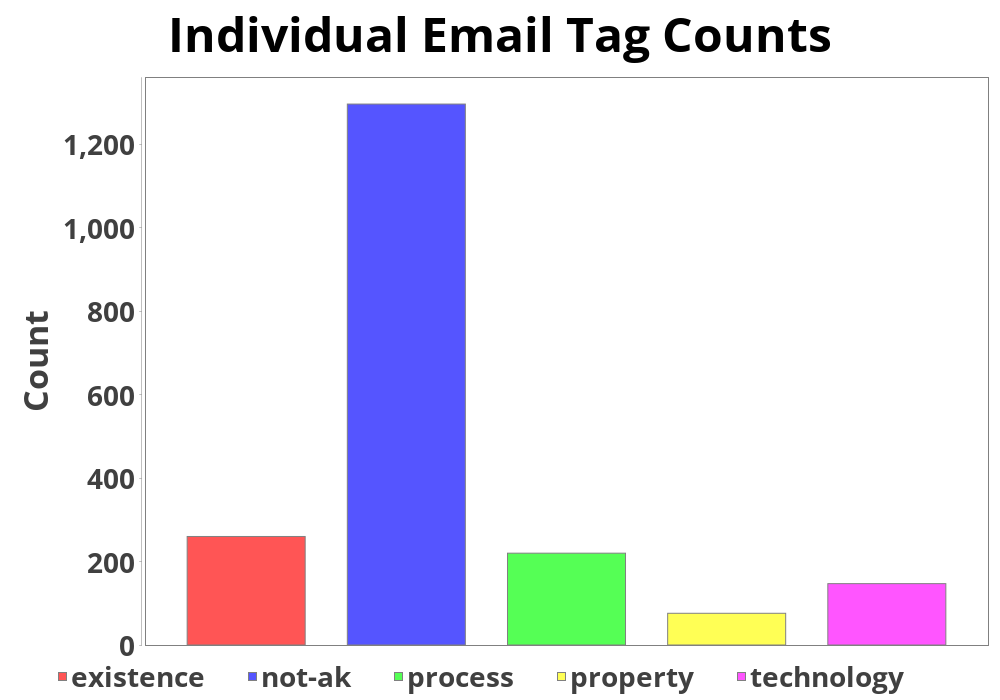
\includegraphics[width=0.7\textwidth]{report/email_tag_counts.png}
			\caption{The total number of emails with each type of tag.}
			\label{fig:emailtagcount}
		\end{figure}
	
		From figure \ref{fig:emailtagcount} we can clearly see that the majority of emails contain no architectural knowledge at all, and by a large margin. However, we also see some interesting variation in what kinds of architectural design decisions do exist, with existence being the most common, followed closely by process decisions.
	
		Looking at the results for threads in figure \ref{fig:threadtagcount}, the outlook isn't quite so depressing. Despite the fact that yet again, \textit{most} threads generally don't have architectural knowledge, a large portion of threads \textit{do} contain a significant number of identified design decisions. Again, existence decisions are the most popular, but thereafter it is evident that there is a relatively large number of threads discussing technology decisions, while fewer process discussions than one would expect if extrapolating the individual email data.
	
		\begin{figure}[H]
			\centering
			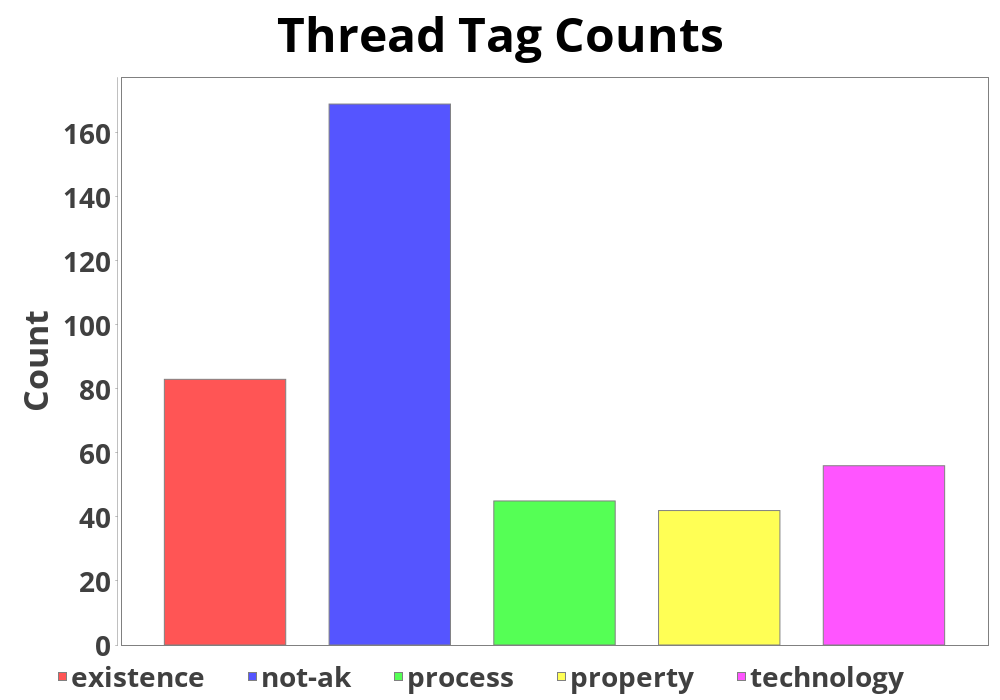
\includegraphics[width=0.7\textwidth]{report/thread_tag_counts.png}
			\caption{The total number of threads that contain each at least one email with a given tag.}
			\label{fig:threadtagcount}
		\end{figure}
	
		The reduced frequency of process discussions at the thread level, juxtaposed with the increased frequency at the individual email level, indicates that there exists a fewer number of threads discussing development processes, \textit{but} those threads which \textit{do} discuss processes, generally contain more emails. We can see this difference illustrated further in figure \ref{fig:threadsize}, which plots the distribution of thread sizes for threads containing various tags.
		
		\begin{figure}
			\centering
			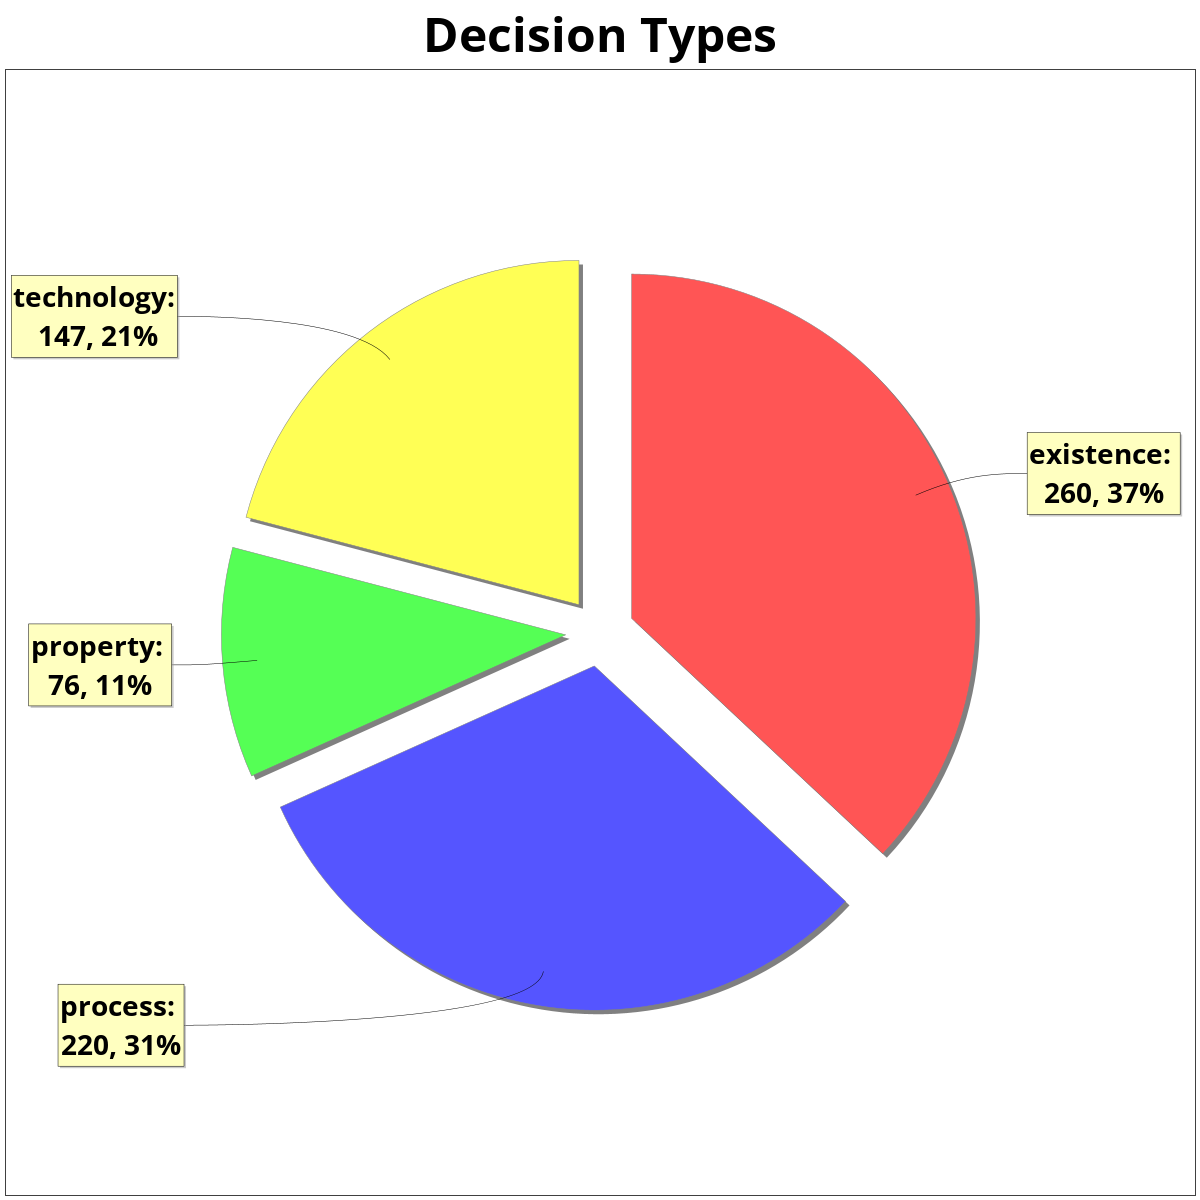
\includegraphics[width=0.7\textwidth]{report/decision_types_pie.png}
			\caption{The relative frequency of the different types of design decisions.}
			\label{fig:decision-types-pie}
		\end{figure}
		
		Conversely, there are proportionately more threads discussing technology than there are individual emails, and again this can be explained by the nature of such discussions. Conversations about technologies tend to be shorter than other conversations about the actual architecture of a system, probably because there is a lesser need to reason about and qualify decisions compared to the system's own components.
		
		\begin{figure}[H]
			\centering
			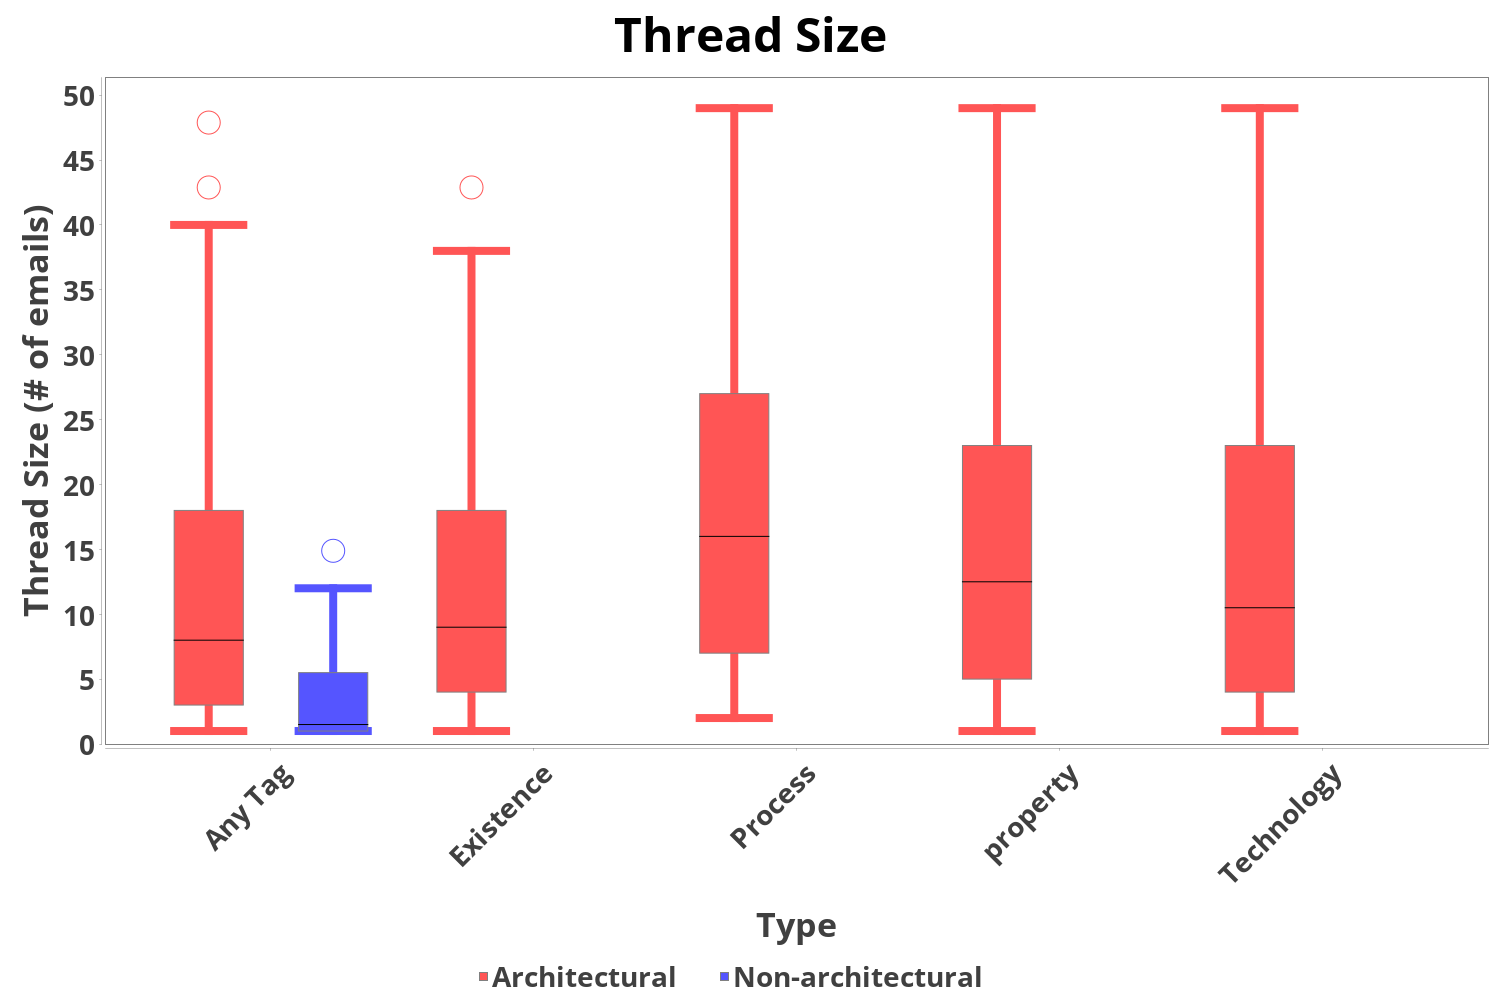
\includegraphics[width=0.8\textwidth]{report/thread_size.png}
			\caption{Boxplot showing the distribution of total thread size for threads containing different tags. A thread is placed into one of the categories if it contains at least one email with that tag.}
			\label{fig:threadsize}
		\end{figure}
	
		\begin{figure}[H]
			\centering
			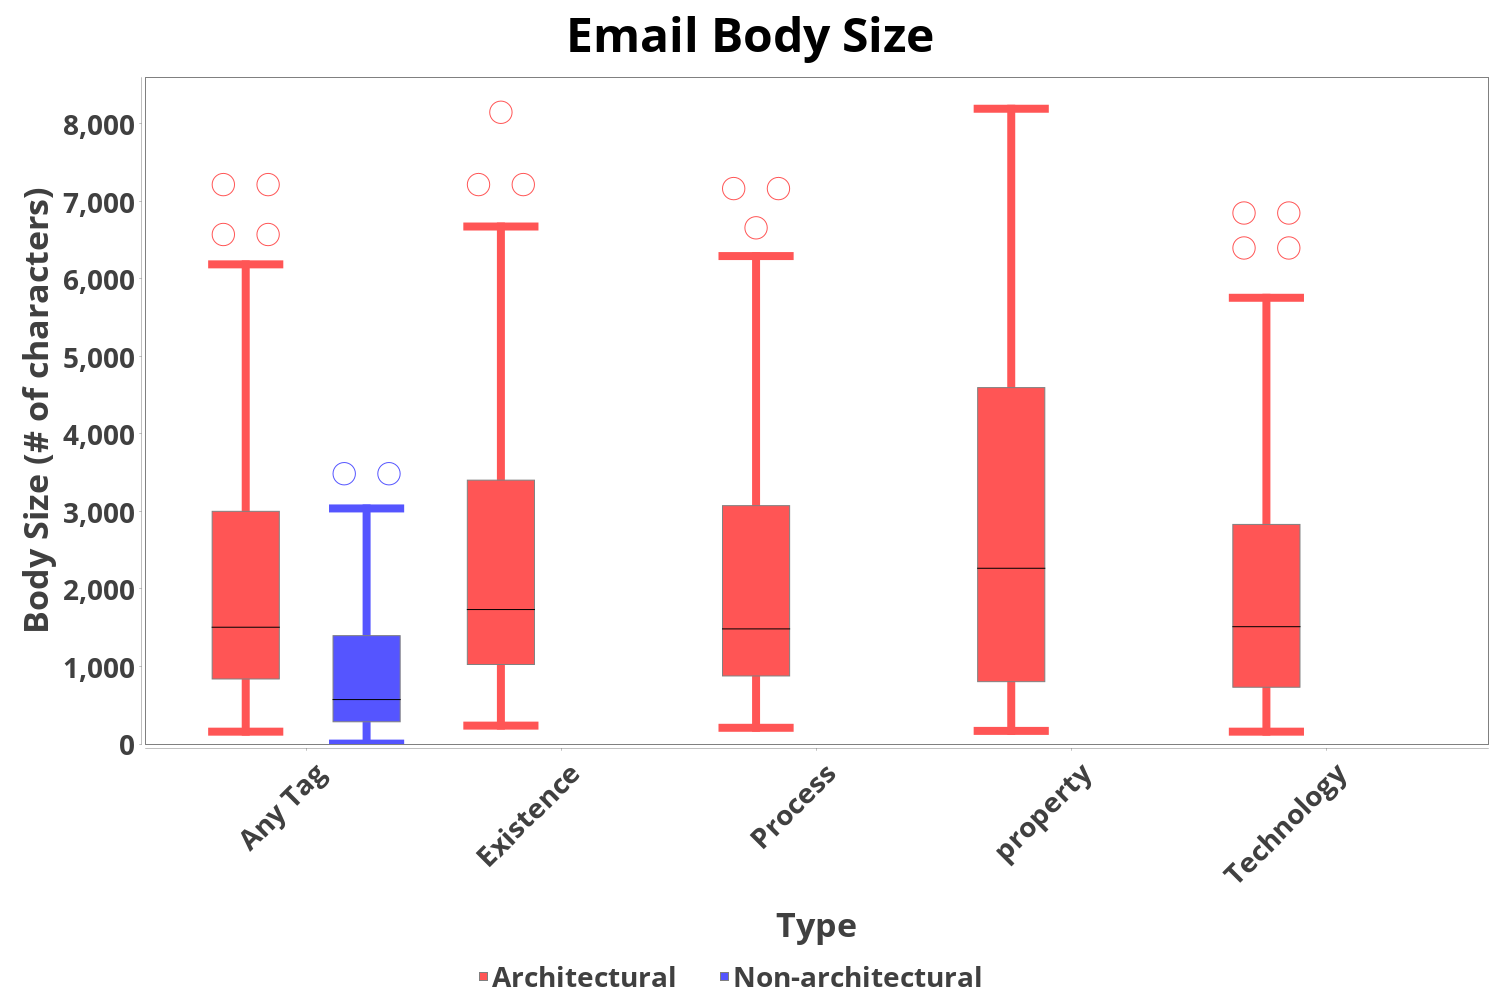
\includegraphics[width=0.8\textwidth]{report/body_size.png}
			\caption{Boxplot showing the distribution of body sizes of emails for threads containing different tags. A thread is placed into one of the categories if it contains at least one email with that tag.}
			\label{fig:bodysize}
		\end{figure}
	
		\begin{figure}[H]
			\centering
			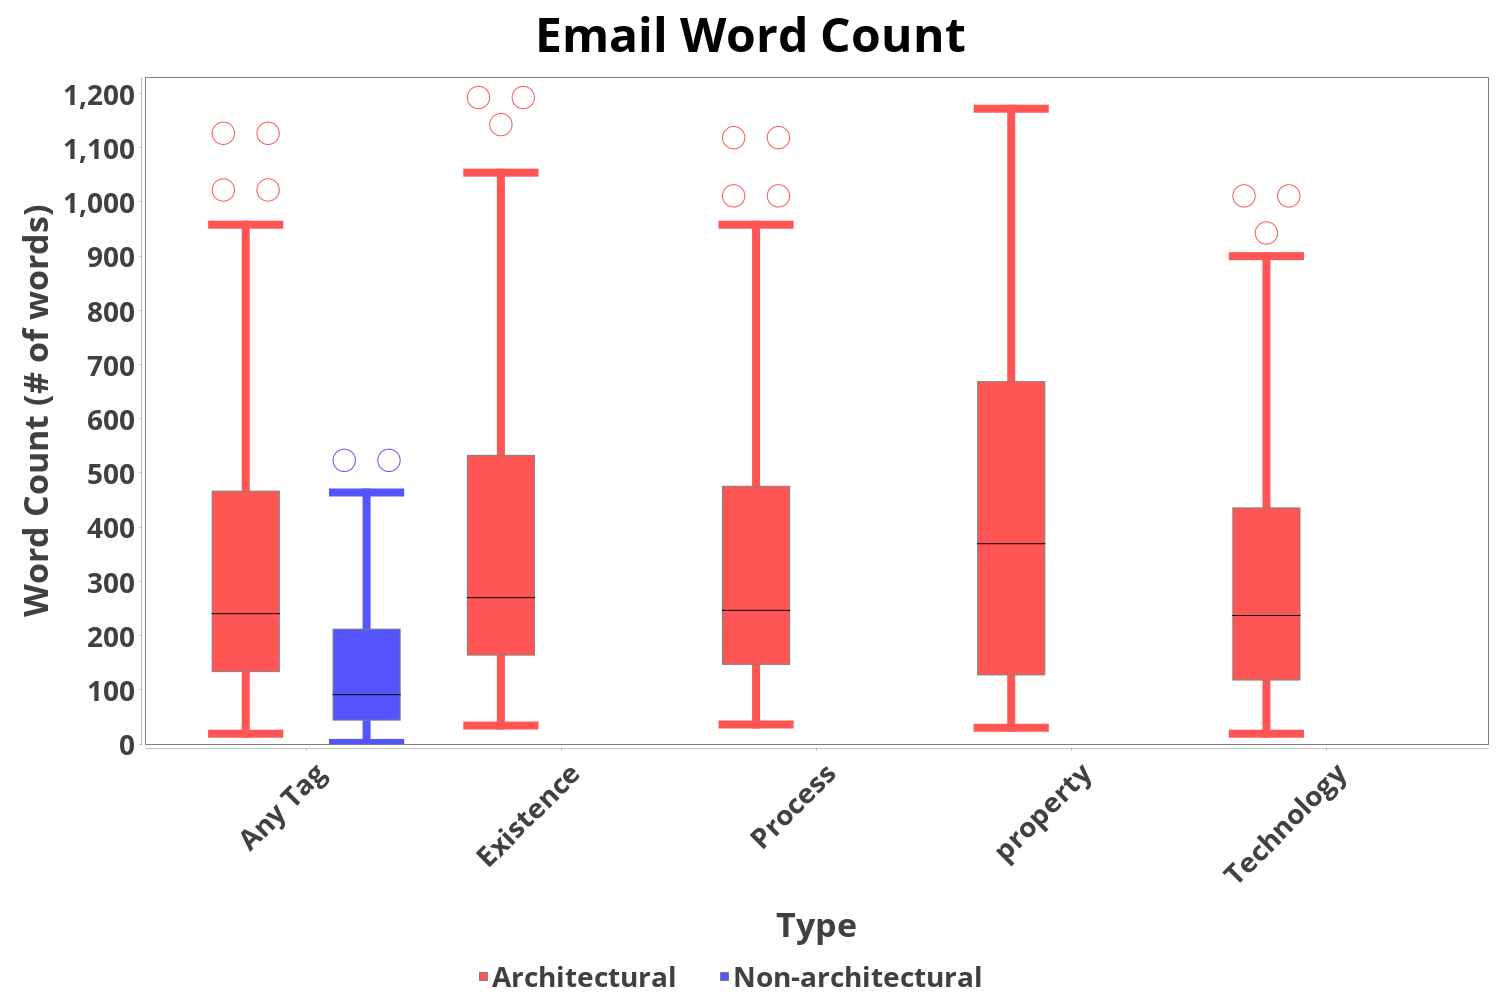
\includegraphics[width=0.8\textwidth]{report/word_count.png}
			\caption{Boxplot showing the distribution of word counts of emails for different tags.}
			\label{fig:wordcount}
		\end{figure}
		
		The \eqref{eqn:thread-relevance} equation provides some insight into how often architectural knowledge appears. We observe a roughly linear gradient from a relevance of 0.1 to a relevance of 1.0, and again we see that a plurality of email threads are mostly irrelevant in terms of their architectural knowledge content.
		
		\begin{figure}[H]
			\centering
			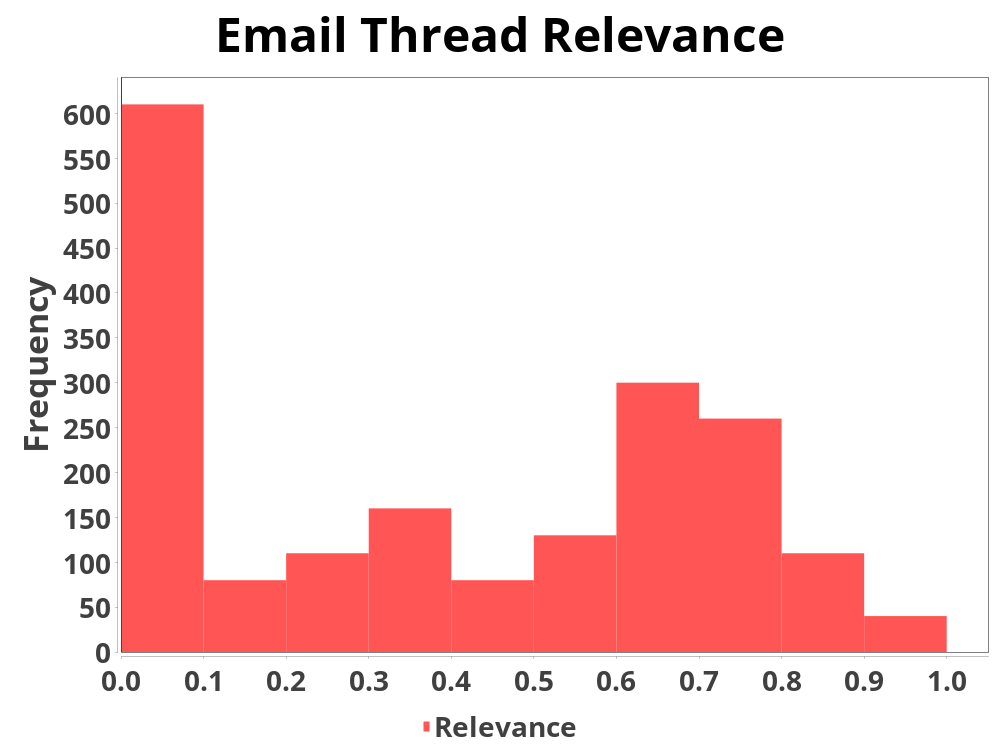
\includegraphics[width=0.7\textwidth]{report/email_thread_relevance_hist.png}
			\caption{Histogram that shows the distribution of the relevance of all email threads.}
			\label{fig:threadrelevance}
		\end{figure}
	
	\subsection{Patterns of Design Decisions}
		To determine if and what sort of patterns exist in progression of architectural design decisions through an email thread, a series of n-gram and co-occurrence analyses were performed. We will first discuss what patterns exist, and then consult a few cases to try and understand why those patterns exist.
		
		\begin{table}[H]
			\centering
			\caption{All 2-gram sequences, ordered from most common to least common.}
			\begin{tabular}{|l|l|}
				\hline
				\textbf{Pattern} & \textbf{Count} \\ \hline
				property    $ \rightarrow $ existence   & 18 \\ \hline
				existence   $ \rightarrow $ process     & 17 \\ \hline
				technology  $ \rightarrow $ existence   & 17 \\ \hline
				existence   $ \rightarrow $ technology  & 16 \\ \hline
				existence   $ \rightarrow $ property    & 15 \\ \hline
				property    $ \rightarrow $ technology  & 14 \\ \hline
				process     $ \rightarrow $ existence   & 11 \\ \hline
				process     $ \rightarrow $ technology  & 11 \\ \hline
				property    $ \rightarrow $ process     & 10 \\ \hline
				technology  $ \rightarrow $ process     & 9 \\ \hline
				technology  $ \rightarrow $ property    & 6 \\ \hline
				process     $ \rightarrow $ property    & 4 \\ \hline
			\end{tabular}
		\end{table}
		
		\begin{table}[H]
			\centering
			\caption{All 2-gram sequences, ordered from most common to least common, skipping non-architectural emails between tags.}
			\begin{tabular}{|l|l|}
				\hline
				\textbf{Pattern} & \textbf{Count} \\ \hline
				existence   $ \rightarrow $ process     & 58 \\ \hline
				existence   $ \rightarrow $ property    & 55 \\ \hline
				technology  $ \rightarrow $ existence   & 54 \\ \hline
				existence   $ \rightarrow $ technology  & 49 \\ \hline
				property    $ \rightarrow $ existence   & 43 \\ \hline
				technology  $ \rightarrow $ process     & 41 \\ \hline
				process     $ \rightarrow $ technology  & 40 \\ \hline
				process     $ \rightarrow $ existence   & 35 \\ \hline
				property    $ \rightarrow $ process     & 27 \\ \hline
				property    $ \rightarrow $ technology  & 25 \\ \hline
				technology  $ \rightarrow $ property    & 21 \\ \hline
				process     $ \rightarrow $ property    & 15 \\ \hline
			\end{tabular}
		\end{table}
	
		Already with just the 2-gram model, it is clear that there is a sort of bidirectional relationship between property and existence decisions, and between existence and technology decisions. Furthermore, the model indicates that there is not a strong directionality in the patterns, since most pairs have a similar frequency with both orientations. The skip-gram technique does lead to more abundant results, but there may be a slightly reduced accuracy\cite{guthrie}, in that an arbitrary number of intermediate emails have been skipped, thus the application of a skip-gram model may not be as reliable as the non-skip, but seems to perform better without needing a larger dataset.
	
		\begin{table}[H]
			\centering
			\caption{Top 5 3-gram sequences, ordered from most common to least common. Other sequences omitted due to low frequency.}
			\begin{tabular}{|l|l|}
				\hline
				\textbf{Pattern} & \textbf{Count} \\ \hline
				property $ \rightarrow $ existence $ \rightarrow $ process & 4 \\ \hline
				existence $ \rightarrow $ property $ \rightarrow $ technology & 3 \\ \hline
				technology $ \rightarrow $ existence $ \rightarrow $ process & 2 \\ \hline
				property $ \rightarrow $ technology $ \rightarrow $ existence & 2 \\ \hline
				property $ \rightarrow $ technology $ \rightarrow $ process & 2 \\ \hline
			\end{tabular}
		\end{table}
		
		\begin{table}[H]
			\centering
			\caption{All 2-gram sequences, ordered from most common to least common, skipping non-architectural emails between tags.}
			\begin{tabular}{|l|l|}
				\hline
				\textbf{Pattern} & \textbf{Count} \\ \hline
				technology  $ \rightarrow $ existence   $ \rightarrow $ process     & 24 \\ \hline
				existence   $ \rightarrow $ process     $ \rightarrow $ property    & 21 \\ \hline
				existence   $ \rightarrow $ property    $ \rightarrow $ process     & 19 \\ \hline
				existence   $ \rightarrow $ technology  $ \rightarrow $ process     & 19 \\ \hline
				technology  $ \rightarrow $ process     $ \rightarrow $ existence   & 19 \\ \hline
				technology  $ \rightarrow $ property    $ \rightarrow $ existence   & 16 \\ \hline
				existence   $ \rightarrow $ technology  $ \rightarrow $ property    & 14 \\ \hline
				property    $ \rightarrow $ existence   $ \rightarrow $ process     & 14 \\ \hline
				existence   $ \rightarrow $ property    $ \rightarrow $ technology  & 13 \\ \hline
				property    $ \rightarrow $ technology  $ \rightarrow $ existence   & 12 \\ \hline
				technology  $ \rightarrow $ existence   $ \rightarrow $ property    & 11 \\ \hline
				process     $ \rightarrow $ technology  $ \rightarrow $ existence   & 10 \\ \hline
				property    $ \rightarrow $ existence   $ \rightarrow $ technology  & 9 \\ \hline
				existence   $ \rightarrow $ process     $ \rightarrow $ technology  & 9 \\ \hline
				property    $ \rightarrow $ technology  $ \rightarrow $ process     & 8 \\ \hline
				technology  $ \rightarrow $ property    $ \rightarrow $ process     & 7 \\ \hline
				process     $ \rightarrow $ existence   $ \rightarrow $ technology  & 7 \\ \hline
				technology  $ \rightarrow $ process     $ \rightarrow $ property    & 6 \\ \hline
				property    $ \rightarrow $ process     $ \rightarrow $ existence   & 6 \\ \hline
				property    $ \rightarrow $ process     $ \rightarrow $ technology  & 3 \\ \hline
				process     $ \rightarrow $ property    $ \rightarrow $ existence   & 3 \\ \hline
				process     $ \rightarrow $ existence   $ \rightarrow $ property    & 2 \\ \hline
				process     $ \rightarrow $ property    $ \rightarrow $ technology  & 1 \\ \hline
				process     $ \rightarrow $ technology  $ \rightarrow $ property    & 0 \\ \hline
			\end{tabular}
		\end{table}
	
		Given that the dataset consists of nearly 2,000 categorized emails, the results of the strict 3-gram model show that there is no abundant evidence for any highly structured patterns of discussion. The skip-gram model offers some more information, but again, the frequencies are quite low to be able to definitively state that a pattern exists. A much larger sample would be needed. Despite that, we do see that technology and existence decisions tend to occur at the beginning of email discussions, while process and property tend to follow.
	
		\begin{table}[H]
			\centering
			\caption{Co-occurrence frequency for pairs of tags.}
			\begin{tabular}{|l|l|}
				\hline
				\textbf{Pattern} & \textbf{Count} \\ \hline
				existence, property & 31 \\ \hline
				existence, technology & 25 \\ \hline
				existence, process & 14 \\ \hline
				process, technology & 9 \\ \hline
				property, technology & 8 \\ \hline
				process, property & 8 \\ \hline
			\end{tabular}
			\label{fig:2co-occurrence}
		\end{table}
	
		The co-occurrence data shown in figure \ref{fig:2co-occurrence} reinforces the previous claim about a relationship between the existence and property decisions, and existence and technology decisions. Now that it is clear that such relationships do exist, we will discuss the possible motivation for the existence of these relationships.
		
		Regarding the existence $ \leftrightarrow $ property relationship, several cases indicate that this happens when a participant begins a high-level proposal or discussion on adding a new component, or integrating a subsystem into the main architecture. This tends to initiate a conversation with one or more property decisions, as users and developers debate on the existing and new properties of the system, and once this is resolved, concrete components or connections between components are proposed.
		
		\subsubsection{Example A}
			An initial email proposes a new implementation of a memtable for the Cassandra project.
			
			\begin{minted}[numbers=none]{text}
We would like to contribute our TrieMemtable to Cassandra.

This is a new memtable solution aimed to replace the legacy implementation, developed with the following objectives:
- lowering the on-heap complexity and the ability to store memtable indexing structures off-heap,
- leveraging byte order and a trie structure to lower the memory footprint and improve mutation and lookup performance.

The new memtable relies on CASSANDRA-6936 to translate to and from byte-ordered representations of types, and CASSANDRA-17034 / CEP-11 to plug into Cassandra. The memtable is built on multiple shards of custom in-memory single-writer multiple-reader tries, whose implementation uses a combination of state-of-the-art and novel features for greater efficiency.
			\end{minted}
		
			This first email is an example of one where existence and property decisions happen together: in this case, the new memtable implementation is a structural change to the architecture, and provides several features that allow better qualitative properties of Cassandra. In a response, we see more existence decisions as the details of the proposed implementation are explained (as these details often imply structural changes to the architecture).
			
			\begin{minted}[numbers=none]{text}
The memtable pluggability API (CEP-11) is per-table to enable memtable selection that suits specific workflows. It also makes full sense to permit per-node configuration, both to be able to modify the configuration to suit heterogeneous deployments better, as well as to test changes for improvements such as this one. 
Recognizing this, the patch comes with a modification to the API that defines memtable templates in cassandra.yaml (i.e. per node) and allows the schema to select a template (in addition to being able to specify the full memtable configuration). One could use this e.g. by adding:
memtable_templates:
	trie:
		class: TrieMemtable
		shards: 16
	skiplist:
		class: SkipListMemtable
memtable:
	template: skiplist 
(which defines two templates and specifies the default memtable implementation to use) to cassandra.yaml and specifying  WITH memtable = {'template' : 'trie'} in the table schema.
			\end{minted}
		
		\subsubsection{Example B}
			In a thread titled \textit{Hadoop Summit: Security Design Lounge Session}, the first email begins by summarizing the attendance and main takeaways from a recent Hadoop Summit meetup, and intends to continue discussion about Hadoop's security in the thread. The author guided the discussion primarily to how to improve Hadoop's security. Already, this identification of points of improvement for the system and preliminary discussion includes property and existence decisions.
			
			\begin{minted}[numbers=none]{text}
...
In order to keep the scope of conversations manageable we tried to keep focused on authentication and the ideas around SSO and tokens.

We discussed kerberos as:
1. major pain point and barrier to entry for some
2. seemingly perfect for others
a. obviously requiring backward compatibility

It seemed to be consensus that:
1. user authentication should be easily integrated with alternative enterprise identity solutions
2. that service identity issues should not require thousands of service identities added to enterprise user repositories
3. that customers should not be forced to install/deploy and manage a KDC for services - this implies a couple options:
	a. alternatives to kerberos for service identities
	b. hadoop KDC implementation - ie. ApacheDS?
...
			\end{minted}
			
			One response to this email provided more support for modifying Hadoop's authentication mechanisms to support pluggable authentication providers, and mentions a third-party authentication provider (ApacheDS) as one example of how it could work.
			
			\begin{minted}[numbers=none]{text}
There was certainly discussions around the emerging work from Daryn related to pluggable authentication mechanisms within that layer and we will immediately have the options of kerberos, simple and plain. There was also talk of how this can be leveraged to introduce a Hadoop token mechanism as well. 

At the same time, there was talk of the possibility of simply making kerberos easy and a non-issue for intra-cluster use. Certainly we need both of these approaches.
I believe someone used ApacheDS' KDC support as an example - if we could standup an ApacheDS based KDC and configure it and related keytabs easily than the end-to-end story is more palatable to a broader user base. That story being the choice of authentication mechanisms for user authentication and easy provisioning and management of kerberos for intra-cluster service authentication.
			\end{minted}
		
	
		In the other common bidirectional case with existence $ \leftrightarrow $ technology, we see a similar pattern of a proposal followed by a rich discussion. For this relationship, however, proposals often directly or indirectly mention third-party technologies, and ensuing conversation includes a series of emails that evaluate the value of integrating such technologies into the architecture.
		
		\subsubsection{Example C}
			In this example, we look at a discussion surrounding the replacement of some old CLI framework used by various Cassandra tools. The current framework (airlift/airline) is deprecated and this email thread is continuing a conversation started in a Slack (instant messaging service) channel.
			
			\begin{minted}[numbers=none]{text}
In CASSANDRA-17445 we’ve started discussing the options of replacing the deprecated airlift/airline framework used in CLI tools.

Considering the amount of commands this framework is used in, the impact this might cause and the future possibilities the operational aspects of Cassandra could leverage, first comments at slack revealed an in-depth discussion would be desirable.

Kind request for comments.
			\end{minted}
		
			The initial message simply expresses a desire to replace the CLI framework, but doesn't provide any specific solutions. This intention to refactor/replace the CLI framework is already an existence decision, as it will generally mean adding and removing some structural components to facilitate a new CLI dependency. Replies go into more detail about actual technologies that can be used to replace the airlift/airline framework.
		
			\begin{minted}[numbers=none]{text}
Maintaining some other tools, originally inspired by nodetool, I started evaluating alternatives. Started with airline2 and picocli, my preliminary findings are

airline2:
+ low effort to replace, nearly unchanged API
+ capability to generate documentation

picocli:
- considerable effort for migration needed
+ more modern and lean API
+ capability to generate documentation
+ capability to generate shell-completion, including not just subcommands but all options and parameters
+ capability to generate man pages

In my opinion, there is room for improvement, especially on documentation and the usability of tools:

* more detailed descriptions on commands and subcommands
* better accessibility to help and docs, e.g. on the website, as man pages, etc.
* adding usage examples to docs and help
* doc pages on the website could be generated e.g. as a side-product of the release process
* the command completion script could be generated, without the need for manual maintenance and packaging
* coloured output in a terminal would be appreciated, especially by less experienced users, e.g. when looking at nodetool status on larger clusters
			\end{minted}
			
			The above reply provides one of the most typical examples of an excellent comparison of technologies, in this case CLI frameworks to use for Cassandra's tools. It also contains a slight property decision, by advocating for the improvement of the tools' usability.
		
			\begin{minted}[numbers=none]{text}
airline/airlift is deprecated. I suspect if there were any security issues they would not be fixed. Their project recommends moving to Airline 2 or picocli.

I share Stefan's concern about the stability of the CLI and output formatting. We should avoid any breakages resulting from this migration. Lots of automation depends on this "interface" being stable.
			\end{minted}
		
			And finally, this reply simply provides a little bit more detail into the motivation behind the desired change.
			
		\subsubsection{Example D}
			In another example, we look at a proposal by a developer for opening Hadoop up to alternative authentication methods beyond just Kerberos (this relates to example B). The initial email provides a list of motivations for why developers should want to do this, and proceeds to ask for community feedback and ideas.
			
			\begin{minted}[numbers=none]{text}
Kerberos was developed decade before web development becomes popular.
There are some Kerberos limitations which does not work well in Hadoop.  A
few examples of corner cases:

1. Kerberos principal doesn't encode port number, it is difficult to know
if the principal is coming from an authorized daemon or a hacker container
trying to forge service principal.
2. Hadoop Kerberos principals are used as high privileged principal, a form
of credential to impersonate end user.
3. Delegation token may allow expired users to continue to run jobs long
after they are gone, without rechecking if end user credentials is still
valid.
4.  Passing different form of tokens does not work well with cloud provider
security mechanism.  For example, passing AWS sts token for S3 bucket.
There is no renewal mechanism, nor good way to identify when the token
would expire.

There are companies that work on bridging security mechanism of different
types, but this is not primary goal for Hadoop.  Hadoop can benefit from
modernized security using open standards like OpenID Connect, which
proposes to unify web applications using SSO.   This ensure the client
credentials are transported in each stage of client servers interaction.
This may improve overall security, and provide more cloud native form
factor.  I wonder if there is any interested in the community to enable
Hadoop OpenID Connect integration work?
			\end{minted}
		
			Another developer responds with more specific information about how they have experience with OpenID Connect (OIDC) authentication.
			
			\begin{minted}[numbers=none]{text}
I'm interested in OpenID Connect (OIDC) integration.

In addition to the benefits (security, cloud native), operating costs may
be reduced in some companies.
We have our company-wide OIDC provider and enable SSO for Hadoop Web UIs
via Knox + OIDC in Yahoo! JAPAN.
On the other hand, Hadoop administrators have to manage our own KDC servers
only for Hadoop ecosystems.
If Hadoop and its ecosystem can support OIDC, we don't have to manage KDC
and that way operating costs will be reduced.
			\end{minted}
		
			This reply provides another motivation for adding support for alternative authentication mechanisms, but mostly motivated by cost optimization rather than just intrinsic benefit of the architecture. This is a common occurrence in technology emails, where respondents qualify their opinions based on the costs of different choices on their industry.
			
			\begin{minted}[numbers=none]{text}
We aren’t very far from having OIDC support.  The pre-requisite RPC/TLS &
RPC/mTLS recently completed rollout to our entire production grid.
Majority of the past year was spent shaking out bugs and ensuring 100%
compatibility.  There are a few rough edges I need to clean up for a
community release.

A few weeks ago I created a rough POC to leverage RPC/mTLS with OIDC access
tokens.  Goal is a mTLS cert may be blessed to impersonate with an access
token.  A compromised service may only be abused to impersonate users that
have recently accessed said service.

Kerberos, mTLs, and OIDC may all be simultaneously supported.  Part of the
simplicity is regardless of the client’s authn/authz, delegation tokens are
still acquired by jobs to avoid short-lived identity credential expiration.
			\end{minted}
			
			And generally, we see multiple emails of a similar nature in technology discussions, where respondents provide their perspective on how they use a technology in their organization, and in the above case, some details about the implementation or how it can be used.
	
	\subsection{Search Effectiveness}
		To determine the effectiveness of our four \hyperref[sec:queries]{queries} at finding relevant emails and threads rich in architectural design decisions, we will use both the \hyperref[eqn:precision]{precision} and \hyperref[eqn:ndcg]{NDCG} as metrics to evaluate over each query.
		
		From figure \ref{fig:precisionall} we can see immediately that all queries generally perform quite well in terms of their precision. Recall that the precision is a measure of the average ratio of returned results that contain architectural knowledge, meaning that all four queries perform slightly above 50\%. Initially, the \textit{decision factors} query performs better, followed by the \textit{rationale} query from $ n = 7 $ onward. The \textit{reusable solutions} and \textit{components and connectors} queries in contrast perform relatively poorly in the initial results, but precision improves as $ n $ approaches 20. However, it should be noted that the initial performance is highly unstable and slight variations in the content of emails may completely alter the first few results, and so practically we should only consider evaluating a query based on its total precision over a greater $ n $.
		
		In figure \ref{fig:ndcgall}, the NDCG metric is visualized for the four queries. The graph is less chaotic than the precision graph, and we can see a more organized trend line for three of queries, while the \textit{reusable solutions} performs consistently at the lowest level. Again, \textit{decision factors} and \textit{rationale} perform well initially, and in this metric, they continue to provide the best performance, albeit by a tiny margin. Despite the fact that the NDCG metric "discounts" results at lower ranks in the result, the queries appear to improve in performance slightly as the result set grows larger. This could indicate that the factor by which we discount lower-ranked results is too weak, or that the queries are simply not effective at ranking highly-relevant results appropriately.
		
		\begin{figure}
			\centering
			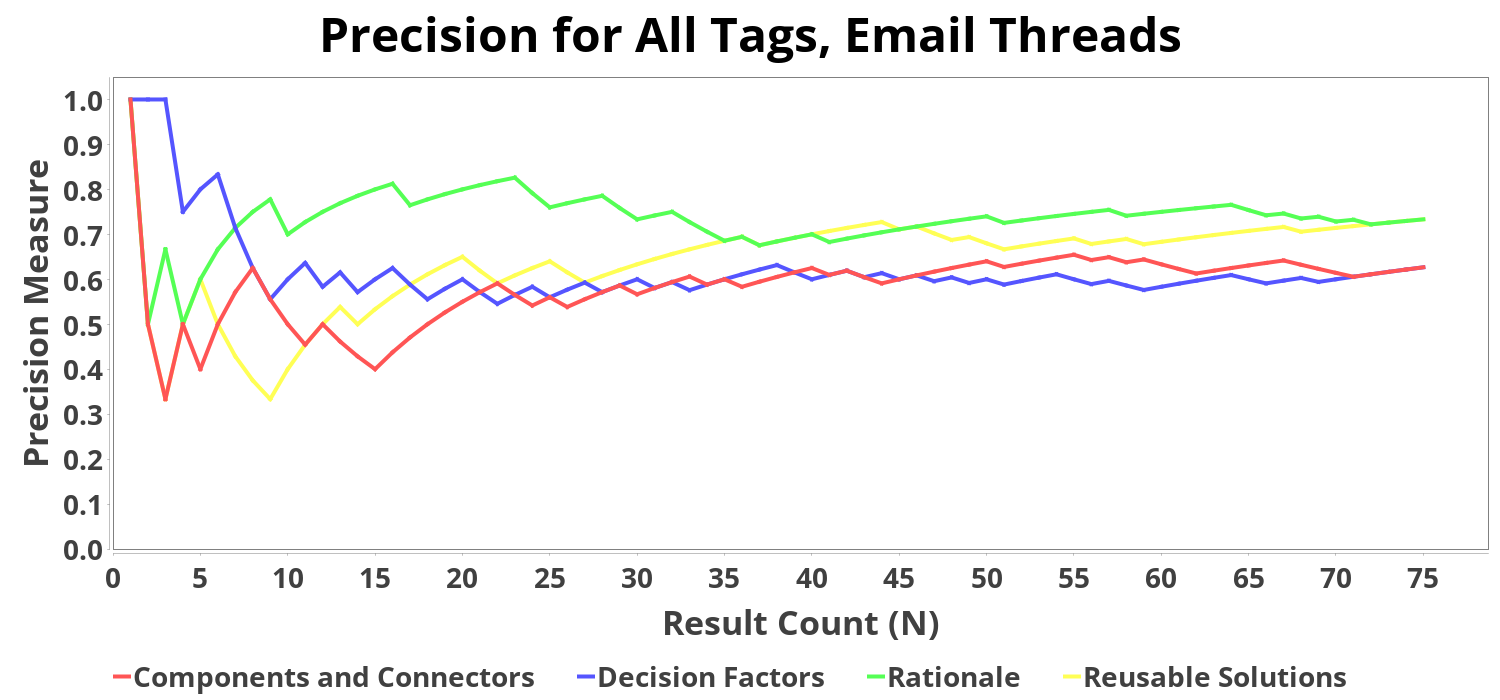
\includegraphics[width=\textwidth]{report/all_tags_thread_precision.png}
			\caption{Precision metric with thread relevance computed using all architectural design decision tags, for all queries.}
			\label{fig:precisionall}
		\end{figure}
		
		\begin{figure}
			\centering
			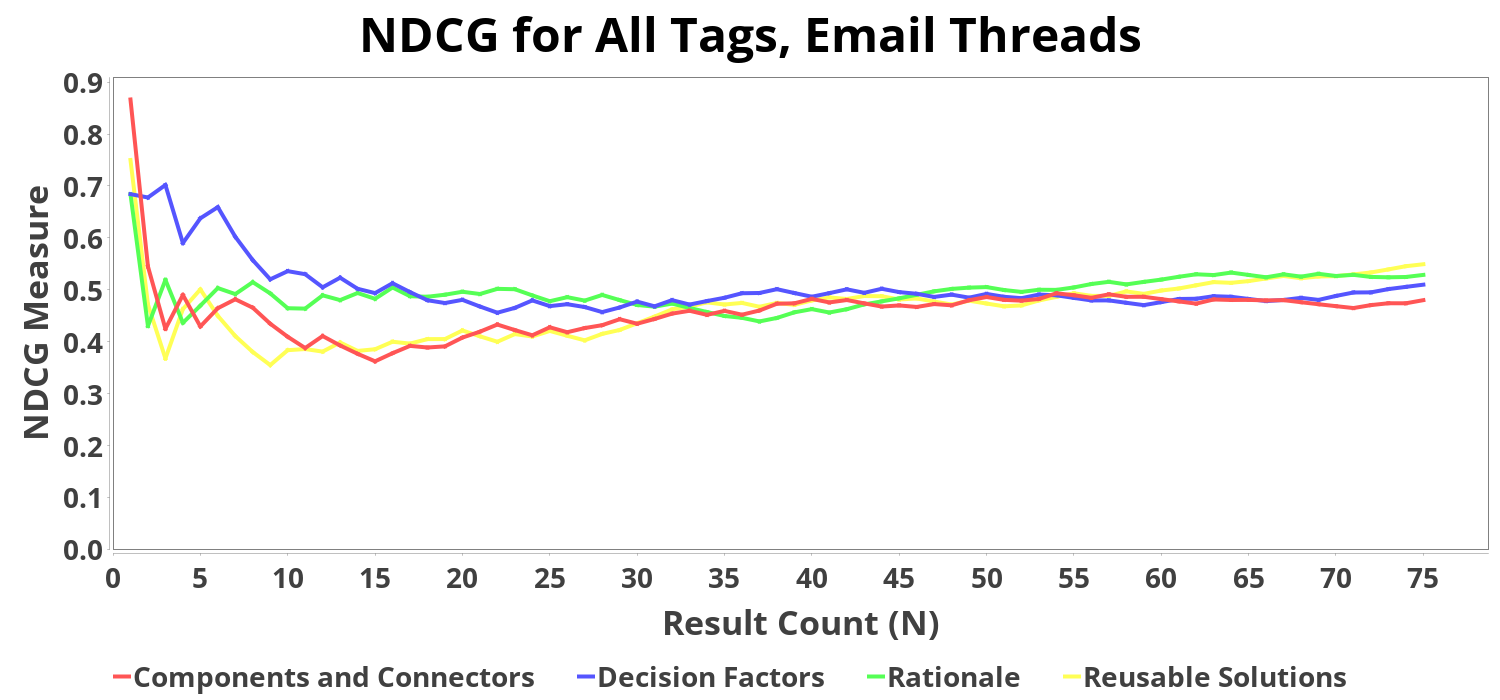
\includegraphics[width=\textwidth]{report/all_tags_thread_ndcg.png}
			\caption{NDCG metric with thread relevance computed using all architectural design decision tags, for all queries.}
			\label{fig:ndcgall}
		\end{figure}
	
		While the focus in this study is on evaluating the effectiveness of queries in a real-world context that's similar to how a user would really search for knowledge, we also include precision and NDCG measures when using the queries to search over individual emails, to compare with the thread-based search. This type of search benefits from a larger dataset volume, as we have roughly 10 times as many fully categorized emails as threads, but does not accurately depict a typical human search, since it removes context from the search results by returning fragmented bits of information from many different conversations. Generally the searches perform worse over individual emails than they do over threads, with both precision and NDCG values remaining below $ 0.4 $ for almost the entirety of the query results, and degrading as $ n $ increases. However, it appears that the \textit{reusable solutions} query, which performed most poorly in the thread-based precision and NDCG metrics, tends to perform at or near the best of all the queries for individual emails.
		
		\begin{figure}
			\centering
			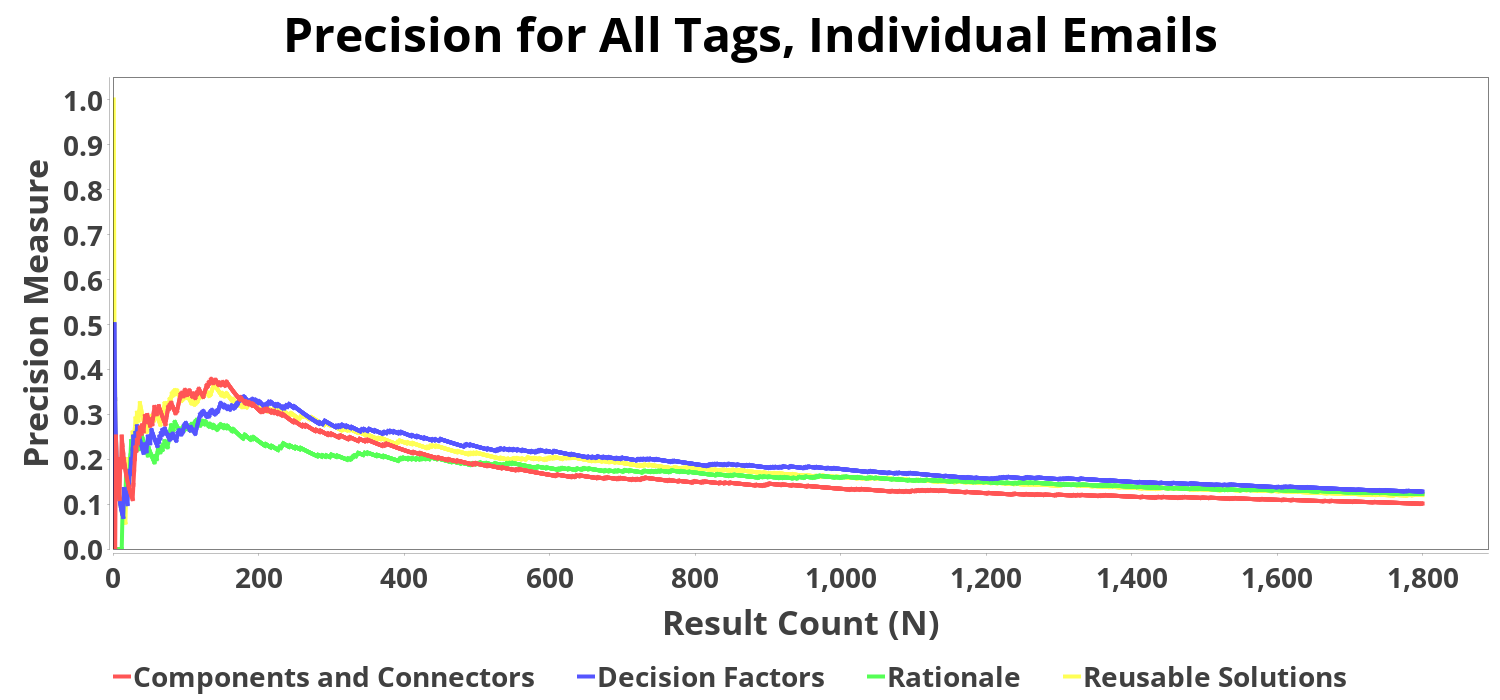
\includegraphics[width=\textwidth]{report/all_tags_email_precision.png}
			\caption{Precision metric with email relevance computed using all architectural design decision tags, for all queries.}
			\label{fig:precisionemailall}
		\end{figure}
		
		\begin{figure}
			\centering
			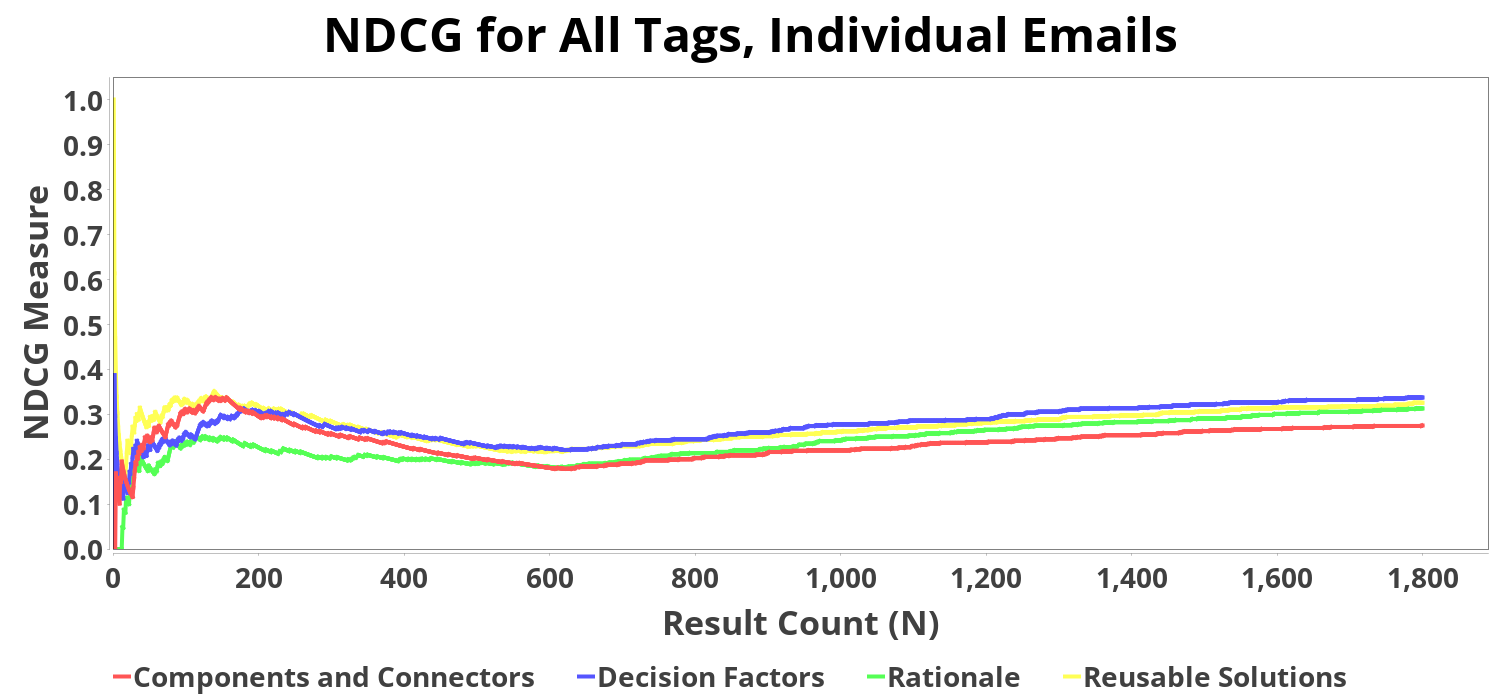
\includegraphics[width=\textwidth]{report/all_tags_email_ndcg.png}
			\caption{NDCG metric with email relevance computed using all architectural design decision tags, for all queries.}
			\label{fig:ndcgemailall}
		\end{figure}

\section{Conclusion}
	In this study, we prepared tools to fetch and process mailing lists, and prepared a categorized dataset containing 1919 emails in 188 unique email threads, to determine what types of architectural knowledge exists in open-source software development mailing lists. The results of a varied set of analyses over this dataset tell us first and foremost that \textit{most} emails in such mailing lists do not contain useful architectural design decisions, but that a large proportion of email threads \textit{do} contain architectural design decisions. There exists a strong relationship between existence decisions and both technology and property decisions, as a natural consequence of the flow of a conversation from proposal to an evaluation of alternative solutions, to choosing an accepted solution.
	
	From applying Apache Lucene search queries to the dataset, the precision and NDCG metrics for both thread-based and individual email results indicate that the current search implementation is not effective for finding a sufficient amount of architectural knowledge, when compared to similar metrics performed by den Boon\cite{denboon} where queries achieved NDCG measures of greater than $ 0.9 $ over 100 results.
	
	Open-source software development mailing lists, as shown by this research, present ample opportunity for extracting architectural knowledge, and we have shown that contextual patterns in the types of design decisions can be used to further aid in searching. However, the search methods used in this study, or the metrics used to grade them, were insufficient to conclude that keyword-based Lucene queries are an effective tool for extracting that knowledge. More work is needed to improve how the queries operate over email threads, how to compute a more accurate relevance measure, and improved metrics are needed to be able to better differentiate the performance of different queries.
	
	\subsection{Threats to Validity}
		Despite the researcher's best efforts, the data in this paper could be subject to a number of faults, and it is important that the reader acknowledge these before pressing onward with any research that depends on these results.
		
		The researcher is a single student whose practical experience does not overlap much with the realm of architectural knowledge identification and extraction. The researcher did iteratively develop a sense of intuition for the design decisions through many weeks of supervised email categorization, but this is still prone to the occasional error. Fatigue may play a role in producing lower-quality results, as multiple hours of reading emails tends to drain the mind of all its vitality.
		
		The indexing and searching implementation may not be optimal for email threads, as no general solution exists for this, given that mailing lists are usually navigated chronologically by their users. The \ref{eqn:thread-relevance} equation may not be optimal for computing a truly useful relevance value for an email thread.
		
	\subsection{Future Work}
		This study provides a solid basis for identifying the types and amount of architectural knowledge that can be found in open-source software development mailing lists, but is far from an exhaustive resource on the matter. Additional research is needed to further expand on the data with additional mailing lists from other open-source communities that focus on different types of software. While we explored the patterns in how architectural design decisions are made, our research was limited to exclusively the content of the emails themselves, and there are many examples where the discussion in an email is migrated to a Jira or GitHub issue tracker, and the reasons for these "jumps" between media has not yet been explored, nor the patterns which might exist between discussions on either end.
		
		While more work can be done to improve the indexing and searching implementation, and the queries used by it, research by Bhat et al.\cite{bhat} shows that there is promise in designing machine learning models to automatically extract architectural knowledge. The data in this study can be incorporated into training data for such models.
		
		The tools developed for this study are rudimentary in nature, but have been developed to the best of the researcher's abilities to be future-proof and open to expansion and re-use, and we encourage others to build on their capabilities. Currently, the \href{https://github.com/ArchitecturalKnowledgeAnalysis/EmailDownloader}{EmailDownloader} utility supports only Apache Software Foundation mailing lists, but could be expanded easily to support others as well. The \href{https://github.com/ArchitecturalKnowledgeAnalysis/EmailIndexer}{EmailIndexer} utility currently only supports the H2 database implementation, which offers limited concurrency when operating in embedded mode, and this can be improved to allow for multi-user systems where many people can contribute to a single dataset's information at once. And finally, the \href{https://github.com/ArchitecturalKnowledgeAnalysis/EmailDatasetBrowser}{EmailDatasetBrowser} application could be expanded to include real-time analytics and improved search interfaces.

\section{References}
	\printbibliography[heading=none]
	\newpage

\section{Appendix}
	This section will contain larger bits of text or code or figures that aren't well suited to being placed inside the body of the paper. They may be referenced throughout the body of the paper. Note that not all source code for the various tools and analyses are included here, due to the impracticality of distributing such a large amount of source code. For the complete suite of software used in this study, please visit the \href{https://github.com/ArchitecturalKnowledgeAnalysis}{ArchitecturalKnowledgeAnalysis} organization on GitHub.
	
	\newpage
	\subsection{Lucene Keyword Queries}
		\label{sec:queries}
		This section contains four keyword-based Lucene search queries provided by Mohamed Soliman, as derived from previous research for use in this project. You may consult \href{https://lucene.apache.org/core/9_2_0/queryparser/org/apache/lucene/queryparser/classic/package-summary.html#package.description}{Apache Lucene's documentation} for a reference of the syntax used in these queries.
		
		\begin{table}[H]
			\begin{tabular}{p{0.4\linewidth} p{0.55\linewidth}}
				Decision Factors &
				\tiny
				\texttt{actor* availab* budget* business case* client* concern* conform* consisten* constraint* context* cost* coupl* customer* domain* driver* effort* enterprise* environment* experience* factor* force* function* goal* integrity interop* issue* latenc* maintain* manage* market* modifiab* objective* organization* performance* portab* problem* purpose* qualit* reliab* requirement* reus* safe* scal* scenario* secur* stakeholder* testab* throughput* usab* user* variability limit* time cohesion efficien* bandwidth speed* need* compat* complex* condition* criteria* resource* accura* complet* suitab* complianc* operabl* employabl* modular* analyz* readab* chang* encapsulat* transport* transfer* migrat* mova* replac* adapt* resilienc* irresponsib* stab* toleran* responsib* matur* accountab* vulnerab* trustworth* verif* protect* certificat* law* flexib* configur* convent* accessib* useful* learn* understand*}
				\\
				Reusable Solutions &
				\tiny
				\texttt{action* adapt* alloc* alternativ* approach* asynch* audit* authentic* authoriz* balanc* ballot* beat bridg* broker* cach* capabilit* certificat* chain* challeng* characteristic* checkpoint* choice* cloud composite concrete concurren* confident* connect* credential* decorat* deliver* detect* dual* echo encapsulat* encrypt* esb event* expos* facade factor* FIFO filter* flyweight* framework* function* handl* heartbeat* intermedia* layer* layoff* lazy load lock* mandator* measure* mechanism* memento middleware minut* monitor* mvc observ* offer* opinion* option* orchestrat* outbound* parallel passwords pattern* peer* period* piggybacking ping pipe* platform* point* pool principle* priorit* processor* profil* protect* protocol* prototyp* provid* proxy publish* recover* redundan* refactor* removal replicat* resist* restart restraint* revok* rollback* routine* runtime sanity* schedul* sensor* separat* session* shadow* singleton soa solution* spare* sparrow* specification* stamp* standard* state stor* strap strateg* subscrib* suppl* support* synch* tactic* task* technique* technolog* tier* timer* timestamp* tool* trail transaction* uml unoccupied* view* visit* vot* wizard* worker*}
				\\
				Components and Connectors &
				\tiny
				\texttt{access* allocat* application* architecture* artifact* attribute* behav* broker* call* cluster* communicat* component* compos* concept* connect* consist* construct* consum* contain* control* coordinat* core criteria* data database* decompos* depend* design* diagram* dynamic element* engine* entit* event* exchang* exist* external filter* function* hardware* independ* information infrastructure input* instance* integr* interac* internal item* job* layer* link* load* logic* machin* memor* messag* model* modul* node* operat* outcom* output* part* peer* platform* port* process* produc* program* project* propert* provid* publish* read* relat* request* resourc* respon* scope separate server* service* shar* source* stor* structur* subscrib* support* system* target* transaction* trigger* runtime realtime network* thread* parallel notif* distribut* backend* frontend* central* persist* queue* concurren* middleware* provid* suppl*}
				\\
				Rationale &
				\tiny
				\texttt{advantag* alternativ* appropriate assum* benefit* better best caus* choic* choos* complex* condition* critical decid* decision* eas* evaluat* hard* quick* rational* reason* risk* simpl* strong* tradeoff weak* rational* disadvantag* comparison* pros cons good differen* slow* lightweight overkill* recommend* suggest* propos* outperform* important* versus vs contrast* distinct* fast* heav* boost* drawback* option*}
				\\
			\end{tabular}
		\end{table}
	
	\newpage
	\subsection{Email Dataset Schema}
		\label{sec:dataset-schema}
		The following SQL snippet defines the relational schema which is used for email datasets in version 2 of EmailIndexer API.
		
		\footnotesize{This DDL script is written using the H2 dialect of SQL.}
		
		\begin{minted}{sql}
CREATE TABLE EMAIL (
	ID BIGINT PRIMARY KEY AUTO_INCREMENT,
	PARENT_ID BIGINT NULL DEFAULT NULL REFERENCES EMAIL(ID)
		ON UPDATE CASCADE ON DELETE SET NULL,
	MESSAGE_ID VARCHAR(255) UNIQUE,
	SUBJECT VARCHAR(1024),
	IN_REPLY_TO VARCHAR(255),
	SENT_FROM VARCHAR(255),
	DATE TIMESTAMP WITH TIME ZONE,
	BODY LONGTEXT,
	HIDDEN BOOL NOT NULL DEFAULT FALSE,
	CHECK (PARENT_ID IS NULL OR PARENT_ID <> ID)
);
CREATE INDEX IDX_EMAIL_DATE ON EMAIL(DATE);
CREATE INDEX IDX_EMAIL_HIDDEN ON EMAIL(HIDDEN);

CREATE TABLE TAG (
	ID INTEGER PRIMARY KEY AUTO_INCREMENT,
	NAME VARCHAR(255) UNIQUE,
	DESCRIPTION MEDIUMTEXT NULL DEFAULT NULL
);
CREATE INDEX IDX_TAG_NAME ON TAG(NAME);

CREATE TABLE EMAIL_TAG (
	EMAIL_ID BIGINT NOT NULL REFERENCES EMAIL(ID)
		ON UPDATE CASCADE ON DELETE CASCADE,
	TAG_ID INTEGER NOT NULL REFERENCES TAG(ID)
		ON UPDATE CASCADE ON DELETE CASCADE,
	PRIMARY KEY (EMAIL_ID, TAG_ID)
);

CREATE TABLE MUTATION (
	ID BIGINT PRIMARY KEY AUTO_INCREMENT,
	DESCRIPTION LONGTEXT NOT NULL,
	PERFORMED_AT TIMESTAMP WITH TIME ZONE NOT NULL DEFAULT CURRENT_TIMESTAMP(0),
	AFFECTED_EMAIL_COUNT BIGINT NOT NULL DEFAULT 0
);
CREATE INDEX IDX_MUTATION_DATE ON MUTATION(PERFORMED_AT);

CREATE TABLE MUTATION_EMAIL (
	MUTATION_ID BIGINT NOT NULL REFERENCES MUTATION (ID)
		ON UPDATE CASCADE ON DELETE CASCADE,
	EMAIL_ID BIGINT NOT NULL REFERENCES EMAIL(ID)
		ON UPDATE CASCADE ON DELETE CASCADE,
	PRIMARY KEY (MUTATION_ID, EMAIL_ID)
);
		\end{minted}
	
	\newpage
	\subsection{Key Analysis Algorithms}
		This section contains a selection of algorithms from the analysis tool which merit their inclusion in this paper.
		
		\subsubsection{N-Gram Pattern Searching}
			\label{sec:pattern-algorithm}
			\begin{minted}{d}
/**
 * Finds a list of sequences of email ids, where the emails in those
 * sequences have tags matching the given pattern of tags, in exactly the
 * same order.
 * Params:
 *   email = The root email to search in.
 *   set = The email set.
 *   pattern = The tag pattern to search for.
 * Returns: A list of email id sequences, where each sequence contains a
 * list of email ids corresponding to emails that have tags matching the
 * given pattern.
 */
private long[][] findMatchingSequences(Email email, EmailSet set, string[] pattern) {
	import std.algorithm;
	import std.array;
	if (pattern.length == 0) return []; // Failsafe exit if the patterns are empty.
	bool thisEmailMatches = email.tags.canFind(pattern[0]);
	long[][] sequences = [];
	// An appender for appending sequences to the list.
	auto sequenceAppender = appender(&sequences);
	if (thisEmailMatches) {
		// Our base case: the root email has a matching tag.
		if (pattern.length == 1) {
			sequenceAppender ~= [email.id];
		} else {
			// Recursive step: find sequences in replies that match the rest of the pattern.
			foreach (reply; set.repliesById[email.id]) {
				foreach (sequence; findMatchingSequences(reply, set, pattern[1 .. $])) {
					sequence.insertInPlace(0, email.id);
					sequenceAppender ~= sequence;
				}
			}
		}
	} else if (skip) {
		// If we allow skipping non-architectural emails, check all replies anyways.
		foreach (reply; set.repliesById[email.id]) {
			sequenceAppender ~= findMatchingSequences(reply, set, pattern);
		}
	}
	return sequences;
}
			\end{minted}
		
		\newpage
		\subsubsection{Thread Relevance}
			\label{sec:thread-relevance-algorithm}
			This set of functions is used to compute the \textit{relevance} of an email thread, in terms of how valuable it is for the thread to appear in search results. See \eqref{eqn:thread-density} and \eqref{eqn:thread-relevance}
			
			\begin{minted}{d}
/** 
 * Computes the relevance of an email thread as a linear combination of the
 * density and relative tag count metrics for the thread.
 * Params:
 *   rootEmail = The root email of the thread.
 *   set = The email set.
 *   akTags = The list of tags which are considered architectural.
 *   maxRelevance = The pre-computed "max" relevance for the set.
 * Returns: The relevance of the thread.
 */
double threadRelevance(Email rootEmail, EmailSet set, string[] akTags, double maxRelevance) {
	import std.algorithm : min;
	uint tagCount = countTagsRecursive(rootEmail, set, akTags);
	return (threadDensity(rootEmail, set, akTags) + min(1.0, tagCount / maxRelevance)) / 2.0;
}

/** 
 * Computes the value that we consider to be the "max relevance" of all email
 * threads in a dataset. This is the third-quartile value of the count of all
 * tags in all email threads.
 * Params:
 *   set = The email set.
 *   akTags = The list of tags which are considered architectural.
 * Returns: The max relevance.
 */
double getMaxRelevance(EmailSet set, string[] akTags) {
	import std.algorithm : sort, mean;
	uint[] rootEmailTagCounts = new uint[set.rootEmails.length];
	foreach (i, rootEmail; set.rootEmails) {
		rootEmailTagCounts[i] = countTagsRecursive(rootEmail, set, akTags);
	}
	rootEmailTagCounts.sort();
	return rootEmailTagCounts[rootEmailTagCounts.length * 3 / 4];
}

/** 
 * Computes the density of an email thread. This is the ratio of architectural
 * emails to the number of total emails in the thread.
 * Params:
 *   rootEmail = The root email.
 *   set = The email set.
 *   akTags = The list of tags which are considered architectural.
 * Returns: The density of the email thread.
 */
double threadDensity(Email rootEmail, EmailSet set, string[] akTags) {
	return cast(double) countAkEmails(rootEmail, set, akTags) / threadSize(rootEmail, set);
}	
			\end{minted}

\end{document}